\documentclass[letter,onecolumn,12pt]{aiaa-tc}

%\usepackage[nolists]{endfloat}
\usepackage{color}
\usepackage[T1]{fontenc}
\usepackage[sc]{mathpazo}
\usepackage{amssymb,latexsym,amsfonts,amsmath}
\usepackage{soul}
\usepackage{url}
%\usepackage{enumitem}
%\usepackage{overpic}
\usepackage{caption}
\usepackage{subfig}
\usepackage{epsfig,psfrag,graphicx,wrapfig}
\usepackage{moresize}
\usepackage{cite}
%\usepackage{hyperref}
%\usepackage[colorlinks,linkcolor=red,urlcolor=green,pagebackref]{hyperref}

\newcommand{\Lone}{\mathcal{L}_1}
\newcommand{\Linf}{\mathcal{L}_{\infty}}
\newcommand{\Lonenorm}[1]{\ensuremath{\left\Vert{#1}\right\Vert_{\mathcal{L}_1}}}
\newcommand{\Linfnorm}[1]{\ensuremath{\left\Vert{#1}\right\Vert_{\mathcal{L}_{\infty}}}}
\newcommand{\Linfnormt}[2]{\ensuremath{\left\Vert{#1}_{#2}\right\Vert_{\mathcal{L}_{\infty}}}}
\newcommand{\lonenorm}[1]{\ensuremath{\Vert{#1}\Vert_{\mathcal{L}_1}}}
\newcommand{\linfnorm}[1]{\ensuremath{\Vert{#1}\Vert_{\mathcal{L}_{\infty}}}}
\newcommand{\linfnormt}[2]{\ensuremath{\Vert{#1}_{#2}\Vert_{\mathcal{L}_{\infty}}}}
\newcommand{\Infnorm}[1]{\ensuremath{\left\Vert{#1}\right\Vert_{\infty}}}
\newcommand{\Twonorm}[1]{\ensuremath{\left\Vert{#1}\right\Vert_{2}}}
\newcommand{\Onenorm}[1]{\ensuremath{\left\Vert{#1}\right\Vert_{1}}}
\newcommand{\Abs}[1]{\ensuremath{\left|{#1}\right|}}
\newcommand{\infnorm}[1]{\ensuremath{\Vert{#1}\Vert_{\infty}}}
\newcommand{\twonorm}[1]{\ensuremath{\Vert{#1}\Vert_{2}}}
\newcommand{\onenorm}[1]{\ensuremath{\Vert{#1}\Vert_{1}}}
\newcommand{\abs}[1]{\ensuremath{|{#1}|}}

\newcommand{\trace}[1]{\ensuremath{{\rm tr}\left({#1}\right)}}
%\newcommand{\Proj}[2]{\ensuremath{{\rm Proj}\left({#1},{#2}\right)}}
\newcommand{\Proj}[3]{\ensuremath{{\rm Proj}_{#1}({#2},{#3})}}
\newcommand{\Exp}[1]{\ensuremath{{\rm e}^{{#1}}}}
\newcommand{\Inv}[1]{\ensuremath{{#1}^{-1}}}

\newcommand{\sech}{\ensuremath{\textrm{sech}}}

\newcommand{\IR}{\mathbb{R}}
\newcommand{\II}{\mathbb{I}}
\newcommand{\thetahat}{\hat{\theta}}
\newcommand{\sigmahat}{\hat{\sigma}}
\newcommand{\omegahat}{\hat{\omega}}
\newcommand{\thetatilde}{\tilde{\theta}}
\newcommand{\sigmatilde}{\tilde{\sigma}}
\newcommand{\omegatilde}{\tilde{\omega}}
\newcommand{\rf}{\mathrm{ref}}
\newcommand{\id}{\mathrm{id}}
\newcommand{\xhat}{\hat{x}}
\newcommand{\xtilde}{\tilde{x}}
\newcommand{\yhat}{\hat{y}}
\newcommand{\ytilde}{\tilde{y}}


\newcommand{\Setups}{\Upsilon_{\omega}}
\newcommand{\underalpha}{\ensuremath{\underline{\alpha}}}
\newcommand{\overalpha}{\ensuremath{\overline{\alpha}}}


\newcommand{\Ccal}{\mathcal{C}}
\newcommand{\Cbarcal}{\bar{\mathcal{C}}}
\newcommand{\Gcal}{\mathcal{G}}
\newcommand{\Hcal}{\mathcal{H}}
\newcommand{\Ical}{\mathcal{I}}
\newcommand{\Kcal}{\mathcal{K}}
\newcommand{\Scal}{\mathcal{S}}
\newcommand{\Tcal}{\mathcal{T}}


\newcommand{\Fao}{F_{\rm a0}(s)}
\newcommand{\Fa}{F_{\rm a}(s)}

\newcommand{\NH}[1]{{\color{red}{#1}}}


%Adjusting quote margins
\renewenvironment{quote}{%
  \list{}{%
    \leftmargin0.5cm   % this is the adjusting screw
    \rightmargin\leftmargin
  }
  \item\relax
}
{\endlist}


%Adjusting description margins
\let\origdescription\description
\renewenvironment{description}{
  \setlength{\leftmargini}{0mm}
  \origdescription
%  \setlength{\itemindent}{0em}
%  \setlength{\labelsep}{\textwidth}
}
{\endlist}

%\newcommand{\matt}[1]{\begin{bmatrix}#1\end{bmatrix}}
%\newcommand{\smatt}[1]{\left[\begin{smallmatrix}#1\end{smallmatrix}\right]}

\graphicspath{{./figures/}}

\renewcommand{\baselinestretch}{0.92}

\begin{document}

\pagestyle{empty}

%\section*{4000-Character Abstract}
%
%The proposed research aims to develop technologies to prevent accidents and incidents resulting from aircraft loss of control~(LOC) as a significant contribution in the ongoing effort to improve the overall safety of the current and future air transportation system. Our proposed framework implements an Integrated Reconfigurable Controller for Vehicle Resilience~(iReCoVeR) that consists of a Resilient Flight Controller, a Flight Envelope Protection system with an LOC Prediction scheme, a Fault Detection and Isolation module, and a Flight Envelope Determination system. With this integrated framework, we address the four subtopics of research topic VSST1-8.
%
%The Resilient Flight Controller is the first line of defense against adverse conditions. The Resilient Flight Controller is a high-performance flight control law designed to provide \emph{short-term stabilization} of the aircraft as well as \emph{improved maneuverability margins} at challenging flight conditions or in the event of moderate faults and failures. The Flight Envelope Protection system ensures that the aircraft stays within its safe operational envelope by overriding, limiting, or shaping the commands generated by the pilot or autopilot. Assisted by the LOC Prediction scheme, it also detects proximity to the boundaries of the envelope and determines the `best' strategy to recover a normal operating condition. The Fault Detection and Isolation module is responsible for detecting and isolating adverse conditions such as sensor failures, vehicle impairment, or ice accretion. Lastly, the Flight Envelope Determination module determines an accurate estimate of the current operational envelope of the possibly impaired aircraft.
%
%In the evaluations of the developed technologies a wide range of adverse conditions will be considered. They will include system failures like sensor failures, vehicle impairment (e.g. due to structural damage and icing conditions), and also external disturbances such as turbulence and wake vortices. Integral part of the proposed work is the development of state-of-the-art aircraft icing models to aid in detection and mitigation of aircraft impairment due to ice accretion. Research will be conducted to obtain both symmetric and asymmetric models of icing accretion, and also extensions will be developed to include unsteady aerodynamic effects due to the coupled effects of the rapid movement of the wing and tail control surfaces with icing. Besides modeling of icing accretion, this research effort also includes the development of methods to detect, isolate, estimate, and mitigate sensor failures, that play a major role in aircraft loss-of-control accidents.
%
%The proposed framework will be designed to perform under a combination of multiple adverse conditions and pilot input errors. Therefore, carefully designed human-in-the-loop experiments will be conducted to evaluate the controller under these challenging conditions. The experiments will be conducted at the human-in-the-loop flight simulation facility at the University of Illinois. The state-of-the-art medium-fidelity flight simulator is highly reconfigurable in both software and hardware. The simulation can be programmed so that specified adverse conditions occur at specified times during flight, and heads-up, heads-down and lateral displays can be added with ease. Part of the validation process is the development of metrics to quantify the nature and magnitude of crew errors leading to an LOC event, as well as the performance during recovery with and without iReCoVeR. Subsequently, the developed iReCoVeR system for LOC prevention will be transitioned to NASA Langley Research Center for implementation on the AirSTAR flight test facility, which provides an actual flight environment to validate the developed technologies.
%
%%\clearpage
%%\thispagestyle{empty}
%%\tableofcontents
%
%\clearpage
%%\pagestyle{plain}
%%\pagenumbering{arabic}


%==============================================================================
\section*{Executive Summary}
%==============================================================================

%------------------------------------------------------------------------------
\textbf{\emph{Objective}:} The proposed research will develop technologies to prevent accidents and incidents resulting from aircraft loss of control~(LOC) as a significant contribution to improve the overall safety of the current and future air transportation system. The proposed framework is an Integrated Reconfigurable Controller for Vehicle Resilience~(iReCoVeR) that consists of a Resilient Flight Controller, a Flight Envelope Protection system with an LOC Prediction scheme, a Fault Detection and Isolation module, and a Flight Envelope Determination system. The technical challenges that will be addressed with iReCoVeR are the four subtopics of VSST1-8:
\begin{itemize}
\setlength{\itemsep}{-4pt}
\vspace{-2mm}
    \item detection of upset onset in the presence of crew input errors and adverse conditions,
    \item prediction of proximity to LOC conditions,
    \item estimation of dynamic flight envelope and upset prevention, and
    \item mitigation of multiple hazards and upset recovery under two or more hazards.
\end{itemize}


%--------------------------  FIGURE  ------------------------------------------
\begin{wrapfigure}{r}{0.63\textwidth}
\centering
%\large
%
\psfrag{LOC}[cc][cc]{{\sf LOC}}
\psfrag{Prediction}[cc][cc]{{\sf Prediction}}
%
\psfrag{Stability}[cc][cc]{{\sf Flight}}
\psfrag{Envelope}[cc][cc]{{\sf Envelope}}
\psfrag{Protection}[cc][cc]{{\sf Protection}}
\psfrag{Determ}[cc][cc]{{\sf Determination}}
%
\psfrag{FDI}[cc][cc]{{\sf FDI}}
\psfrag{Module}[cc][cc]{{\sf Module}}
%
\psfrag{RFC}[lc][lc]{{\sf Resilient Flight Control}}
\psfrag{L1}[cc][cc]{{\sf $\Lone$ Adaptive}}
\psfrag{Aug}[cc][cc]{{\sf Augmentation}}
\psfrag{Baseline}[cc][cc]{{\sf Baseline}}
\psfrag{Controller}[cc][cc]{{\sf Controller}}
%
\psfrag{RFTC}[lc][lc]{{\sf iReCoVeR}}
%
\psfrag{fdi}[lc][lc]{{\sf \it FDI}}
\psfrag{trigger}[lc][lc]{{\sf \it trigger}}
%
\psfrag{reconf}[lc][lc]{{\sf \it reconfig.}}
%
\psfrag{pilot}[cr][cr]{{\sf \it pilot/autopilot}}
\psfrag{command}[cr][cr]{{\sf \it command}}
\psfrag{u}[cl][cl]{{\sf \it control}}
\psfrag{signal}[cl][cl]{{\sf \it signal}}
\psfrag{yh}[cl][cl]{{\sf \it feedback}}
%
\vspace{-4mm}
\includegraphics[angle=-90,width=0.6\textwidth,]{irecover.ps}
\caption*{\footnotesize iReCoVeR: \textbf{I}ntegrated \textbf{Re}configurable \textbf{Co}ntrol for \textbf{Ve}hicle \textbf{R}esilience.}
\label{fig:IReCoVeR}
\end{wrapfigure}
%------------------------------------------------------------------------------

\vspace{-1mm}
Research will build upon past expertise with the AirSTAR flight test facility and the use of $\Lone$~adaptive control to ensure a predictable response to the pilot in the presence of adverse conditions. The iReCoVeR system will be designed to perform under a combination of multiple adverse conditions and pilot input errors. The adverse conditions include system failures (like sensor and actuator failures), vehicle impairment, turbulence, and wake vortices. Special emphasis will be placed on sensor failures and adverse icing conditions. The developed solutions will be first validated on a full-scale aircraft model in the flight simulator of the University of Illinois's Beckman Institute with a pilot in the loop, and later transitioned to the facilities of NASA~LaRC. We will seek to establish theoretically valid guidelines for the design of next generation flight control systems through collaborative efforts with our partners at NASA LaRC and University of Connecticut.


\medskip

%------------------------------------------------------------------------------
\textbf{\emph{Expected Outcomes and Benefits}:} The expected outcome from this research effort is the iReCoVeR system (depicted in the figure). The following algorithms will be developed: $(i)$~algorithms for detection and isolation of adverse conditions that are able to identify a model of the possibly impaired aircraft; $(ii)$~estimation and control algorithms to estimate and protect the flight envelope; and $(iii)$~prediction algorithms to assess the proximity of the aircraft to an LOC event. The main benefit will be a \emph{safer} flight control system as envisioned under the NextGen concept in the 2025 time frame.


\medskip

%------------------------------------------------------------------------------
\textbf{\emph{Relevance to NASA Strategic Plan}:} The proposed research assures safe operation under the current air transportation system and the NextGen concept through prediction and prevention of LOC. In particular, the proposed framework addresses the four subtopics of \mbox{VSST1-8}, which is part of the Research project ``Vehicle Systems Safety Technologies Project''~(B3) and announced by the NASA Aeronautics Research Mission Directorate in support of NASA Strategic Goal~4 and Outcome~4.1.




%==============================================================================
\section{Objectives and Significance of the Proposed Research}
%==============================================================================

The main objective of this research effort is to develop technologies to prevent accidents and incidents resulting from aircraft loss of control~(LOC) as a significant contribution in the ongoing effort to improve the overall safety of the current and future air transportation system. To date, aircraft LOC is still the major cause of all fatal aircraft accidents~\cite{LOC04_LOCMetrics,LOC_2007,MST08_upsets,LOC_2010,LOC10_Belcastro_analysis,LOC10_Belcastro_concept}. The proposed framework is an Integrated Reconfigurable Controller for Vehicle Resilience~\mbox{(iReCoVeR)} that consists of a Resilient Flight Controller, a Flight Envelope Protection system with an LOC Prediction scheme, a Fault Detection and Isolation module, and a Flight Envelope Determination system. The technical challenges that will be addressed with the iReCoVeR system are the four subtopics of VSST1-8:
\begin{itemize}
\setlength{\itemsep}{-3pt}
\vspace{-2mm}
    \item detection of upset onset in the presence of crew input errors and adverse conditions,
    \item prediction of proximity to LOC conditions,
    \item estimation of dynamic flight envelope and upset prevention, and
    \item mitigation of multiple hazards and upset recovery under two or more hazards.
\end{itemize}
In the evaluations of the developed technologies a wide range of adverse conditions will be considered. They will include system failures like sensor and actuator failures, vehicle impairment (e.g. due to structural damage and icing conditions), and also external disturbances such as turbulence and wake vortices. The iReCoVeR system will be designed to perform under a combination of multiple adverse conditions and pilot input errors. Therefore, carefully designed human-in-the-loop experiments will be conducted to evaluate the controller under these challenging conditions. Special emphasis will be placed on sensor failures and adverse icing conditions.


As part of long term Strategic Goal~4~\cite{NASA_goals11}, NASA is developing solutions to challenges arising from the Next Generation Air Transportation System~(NextGen).
 %One of the greatest challenges is to assure safe operation of air transportation at all times, while enabling airspace capacity expansion and optimization through increased automation onboard aircraft, necessary due to the expected rapid growth of air travel over the next decade.
%Not only will the proliferation of sophisticated automation onboard aircraft allow tighter separation to inclement weather, terrain, and other aircraft, it will also enable all-weather operations. It is also envisioned that piloted aircraft and fully-automated unmanned aircraft systems will operate side-by-side in the same airspace.
%It is expected that any occurrence of LOC within the NextGen will have catastrophic effects due to the increased density of aircraft and closer spacing to terrain. Hence,
Prevention of LOC is a key challenge to overcome in order to ensure safe operation under the NextGen. The proposed work makes a leap toward achieving this goal. In particular, this research supports in achieving Outcome~4.1 through addressing Objective~4.1.1 as stated in~\cite{NASA_goals11}.


The research project ``Vehicle Systems Safety Technologies Project''~(B3) that is announced by the NASA ARMD attempts to ``identify vehicle-related risks and develop technologies needed to avoid, detect, mitigate, and recover from hazardous flight conditions, and to maintain vehicle airworthiness and health''. One of the three identified key technical challenges is assuring safe and effective aircraft control under hazardous conditions~\mbox{(TC-3)}. Research topic~VSST1-8 seeks solutions addressing~TC-3. This proposed research will address all four subtopics that are outlined under VSST1-8.


%==============================================================================
\section{Technical Approach and Methodology: iReCoVeR}
%==============================================================================

%------------------------------------------------------------------------------
\subsection{Motivation and Background}
%------------------------------------------------------------------------------

LOC accidents remain a major cause of fatal accidents across all vehicle classes and operational categories. American Airlines Flight~587's fatal accident in New~York is an example of an accident that is classified as an LOC accident~\cite{MST08_upsets}. The aircraft crashed into Belle Harbor,~NY, shortly after takeoff from JFK~International Airport on November~12, 2001. Flight~587 was caught in the wake of a Boeing 747 and the first officer attempted to stabilize the aircraft by applying large and aggressive alternating inputs to the rudder, that eventually caused the vertical stabilizer to break off mid-air. Official investigations concluded that if the first officer had ceased all additional inputs to the rudder, the aircraft would have stabilized, and the fatal accident could have been prevented.


On October~31, 1994 an ATR-72 operated by American Eagle crashed in Roselawn,~IN, killing all 64~passengers and 4~crew members onboard. While holding at 10,000~ft, Flight~4184 encountered icing conditions that turned out to be fatal. After clearance was given, the pilots initiated their descend into O'Hare International Airport. Two sudden uncommanded rolls sent the aircraft into an LOC. The NTSB concluded that ``the probable cause of this accident were the loss of control, attributed to a sudden and unexpected aileron hinge moment reversal that occurred after a ridge of ice accreted beyond the deice boots''~\cite{ATR72}.


A more recent accident involved an Air France Airbus~A330 en-route from Rio de Janeiro to Paris on June~1, 2009. The aircraft plunged into the Atlantic Ocean due to what seems to have initiated from an inconsistent airspeed sensor reading. Preliminary investigations showed that most likely icing inside the pitot tubes was the cause of the erroneous airspeed readings, which led to the automatic disengagement of the autopilot. Unfortunate combination of spatial disorientation of the crew and miscommunication between the pilots, seemed to have caused the aircraft to stall due to high angles of attack of 40~degrees. At that time, the aircraft was descending at a dazzling rate of nearly 11,000~ft per minute and eventually crashed into the Atlantic Ocean. Official conclusions of the investigations are still pending publication.


The examples illustrate that there is no clear and seldom single cause for an aircraft LOC event, but rather it can result from a wide range of causal and contributing factors that occur individually or in combination sequentially in time. These factors can be categorized as adverse conditions occurring onboard the vehicle, external hazards and disturbances, and aircraft upset conditions~\cite{LOC10_Belcastro_concept}. Reference~\cite{MST08_upsets} provides a definition of aircraft upset condition as ``any uncommanded or inadvertent event with an abnormal aircraft attitude, rate of change of aircraft attitude, acceleration, airspeed, or flight trajectory''. The same reference also notes that ``abnormal'' must be determined relative to phase flight and aircraft type.


Prevention of LOC accidents becomes even more crucial in future airspace operations under the NextGen Air Transportation System~\cite{NextGen_ConOps}. The NextGen provides a vision of highly integrated airspace operations in the 2025 time frame, necessary in order to cope with the rapid growth of air travel and operational diversity. The NextGen concept of operations includes high-density, all-weather, and self-separation operational concepts, and is also expected to allow mixed-capability aircraft to operate within the same airspace, including piloted aircraft and unmanned aircraft systems. Potential future LOC risks may emerge as for example increased onboard automation allows all-weather operations combined with highly precise trajectories that enable closer spacing to inclement weather, terrain, and other aircraft. These developments might increase the likelihood of the occurrence of LOC events and hence onboard integrated systems technologies for LOC prediction and prevention will be of paramount importance to future safety critical avionics systems.


Before a solution can be formulated, it is necessary to obtain a quantitative definition of LOC that is generally accepted among the investigators and researchers in this area.
%Traditionally, LOC has been described in qualitative terms as a motion that is outside the normal operating flight envelopes, not predictably altered by pilot control inputs, characterized by nonlinear effects, likely to result in high angular rates and displacements, and characterized by the inability to maintain heading, altitude, and wings-level flight~\cite{LOC04_LOCMetrics}. Based on these characteristics of an LOC event it is evident that there is a need to transcribe this information into measurable quantities.
The authors of~\cite{LOC04_LOCMetrics} approached the problem from a flight dynamics perspective and developed metrics in terms of parameters such as angle of attack, airspeed, pitch attitude, pitch rate, sideslip, and bank angle, among others. The metrics, known as the Quantitative Loss-of-Control Criteria, are composed of five envelopes relating to the airplane flight dynamics, aerodynamics, structural integrity, and flight control use. Applying these metrics to data from LOC events, the authors concluded that an excursion of three or more envelopes is a reliable, quantitative indication of LOC. These generally accepted metrics will be used in the proposed research to quantify, identify, and predict LOC~events.


Due to the convoluted character of the contributing factors and the string of events leading to aircraft upset and ultimately to an LOC event, there will be no one-stop-solution that prevents all LOC accidents. In contrary there is a need for parallel approaches to address prevention~\emph{and} recovery from these upsets~\cite{MST08_upsets}. Reference~\cite{LOC10_Belcastro_concept} takes a holistic perspective in approaching the problem and puts forward an integrated systems concept for preventing aircraft LOC accidents: the \emph{AIRSAFE System concept}. A detailed description of the AIRSAFE System concept can be found in~\cite{AIRSAFE_part1}.
%The core subsystems and capability include vehicle health management, vehicle flight safety management and resilient control, crew-system interfaces and onboard modeling capability.
The emphasis of AIRSAFE is to arrest the development of an LOC sequence through the core subsystems and the onboard modeling capability, by breaking the sequence at the different stages.


%%--------- FIGURE --------------------------------------------------------------------------------------
%\begin{figure}[h]
%	\centering
%		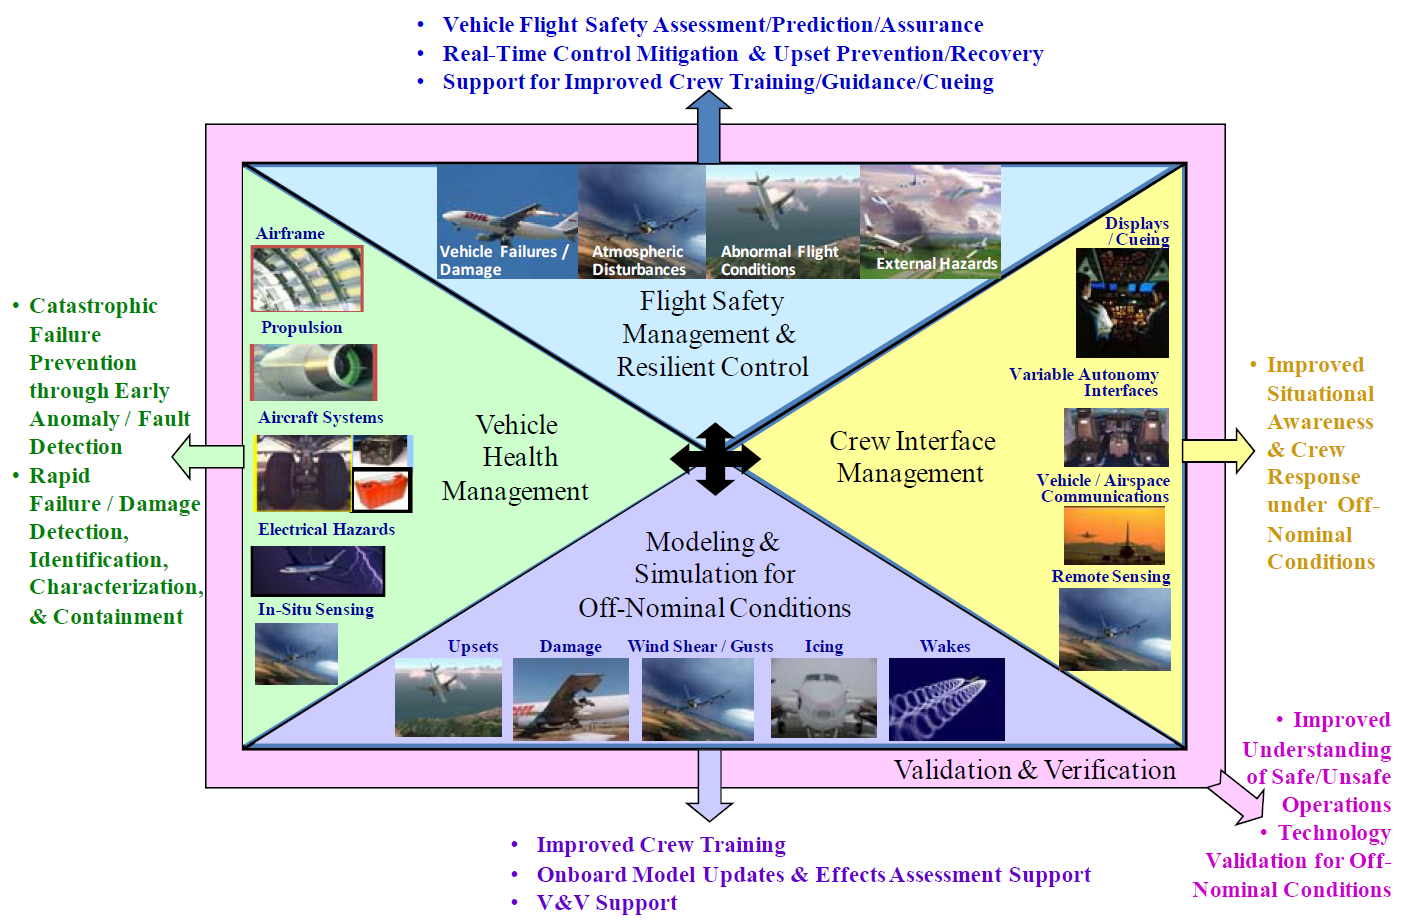
\includegraphics[width=0.70\textwidth]{LOC_holistic_appr.eps}
%	\caption{A holistic approach for preventing aircraft LOC accidents; figure taken from~\cite{LOC10_Belcastro_concept}.}
%	\label{fig:holistic_approach}
%\end{figure}
%%-------------------------------------------------------------------------------------------------------


%Figure~\ref{fig:gen_loc_sequence} shows an example of a generic LOC accident sequence, which is a typical chain of events that is observed from past aircraft LOC accident data.
In a typical LOC accident sequence without a proper intervention strategy~\cite{LOC10_Belcastro_concept}, a vehicle impairment or external hazard might trigger an inappropriate crew response due to for example poor situational awareness. Subsequently, the aircraft may enter an upset condition and eventually result in an LOC event. As proposed with AIRSAFE, the subsystems provide prevention and intervention of the development of an LOC sequence.
%For example, continuous monitoring of the critical aircraft systems by vehicle health management technologies would help to prevent failures and damages from occurring. Improved situational awareness interfaces for the crew would reduce the possibility of inappropriate pilot inputs once a vehicle impairment or external hazard condition has occurred. And lastly, onboard modeling capabilities could update the vehicle health management system on the actual off-nominal condition of the aircraft.
An effective strategy is to intervene at the different stages of a typical LOC sequence by avoiding/detecting vehicle impairment and external hazard conditions, mitigating their effects and recovering from an actual vehicle upset. The AIRSAFE concept describes the necessary subsystems and capabilities that collectively achieve LOC prediction and prevention.


%--------- FIGURE --------------------------------------------------------------------------------------
%\begin{figure}[h]
%	\centering
%        \subfloat[Without onboard intervention systems.]{
%    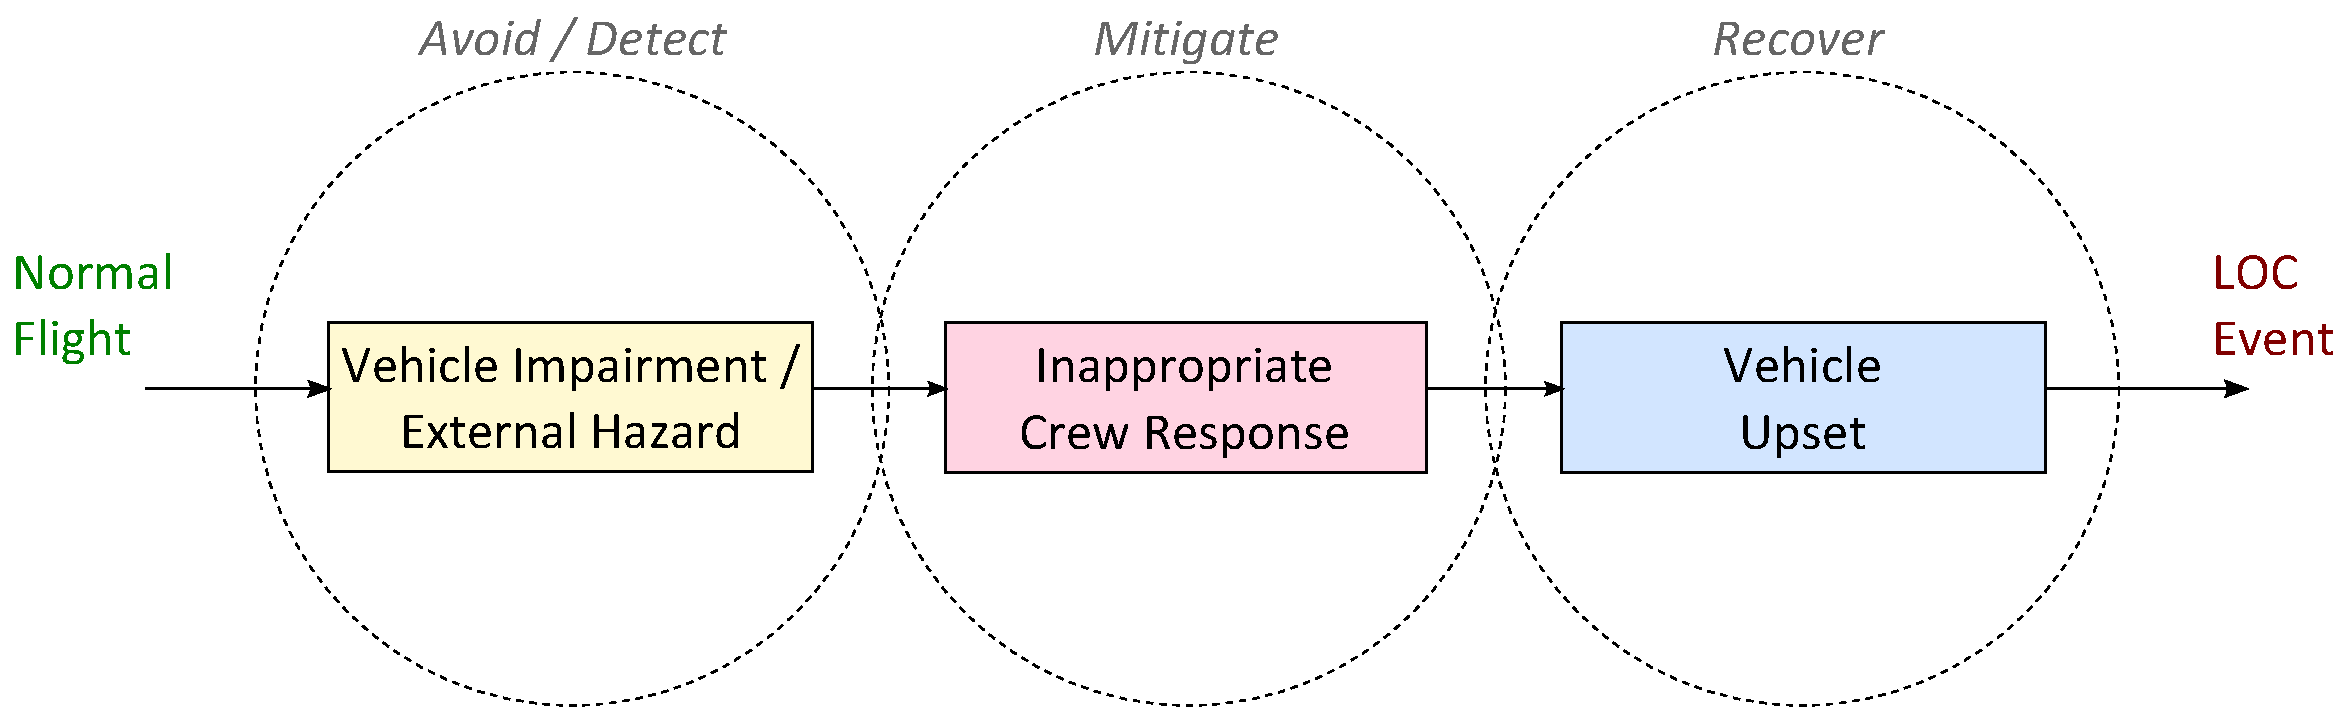
\includegraphics[width=0.5\textwidth]{LOC_accident_sequence.eps}\label{subfig:loc_seq}}\\
%        \subfloat[With onboard intervention systems.]{
%    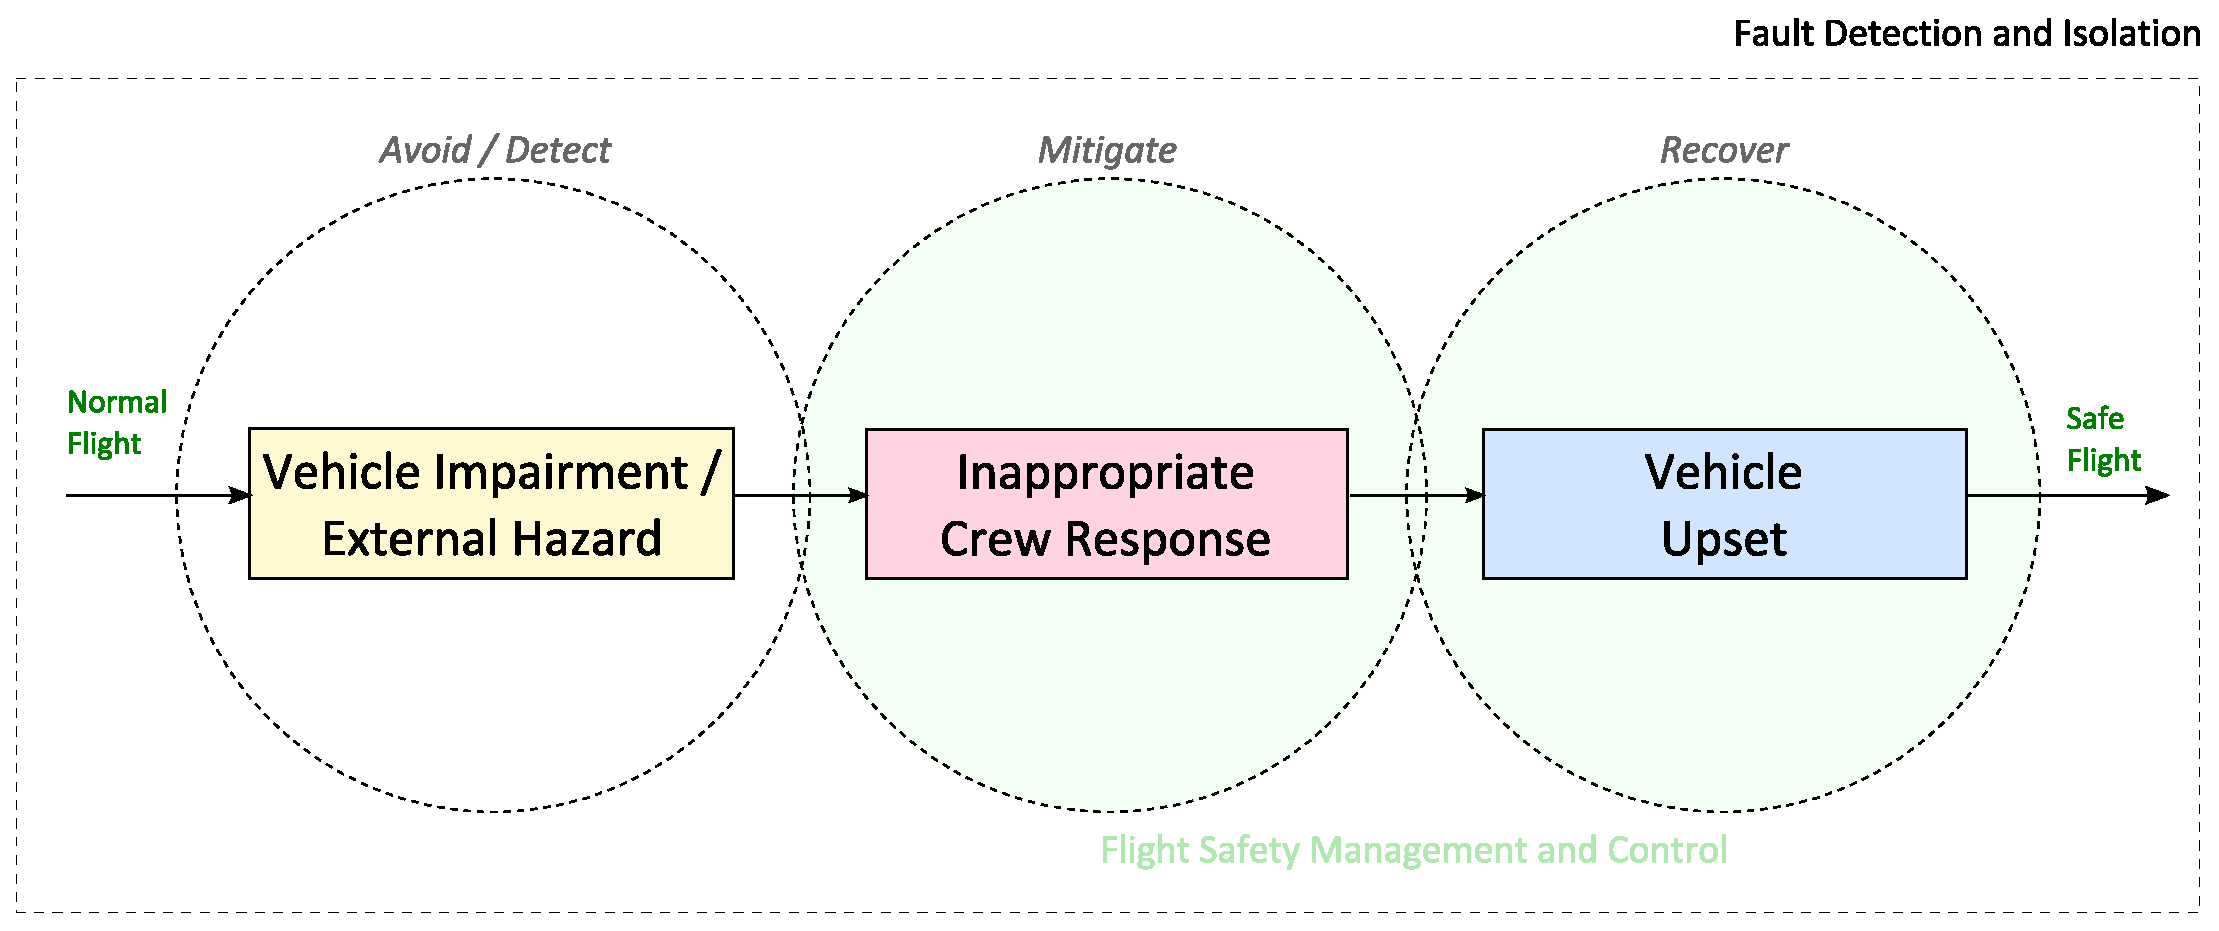
\includegraphics[width=0.5\textwidth]{LOC_accident_sequence_sol.eps}\label{subfig:loc_seq_sol}}
%	\caption{Generic LOC sequence.}
%	\label{fig:gen_loc_sequence}
%\end{figure}
%-------------------------------------------------------------------------------------------------------


%--------- FIGURE --------------------------------------------------------------------------------------
%\begin{figure}[h]
%	\centering
%    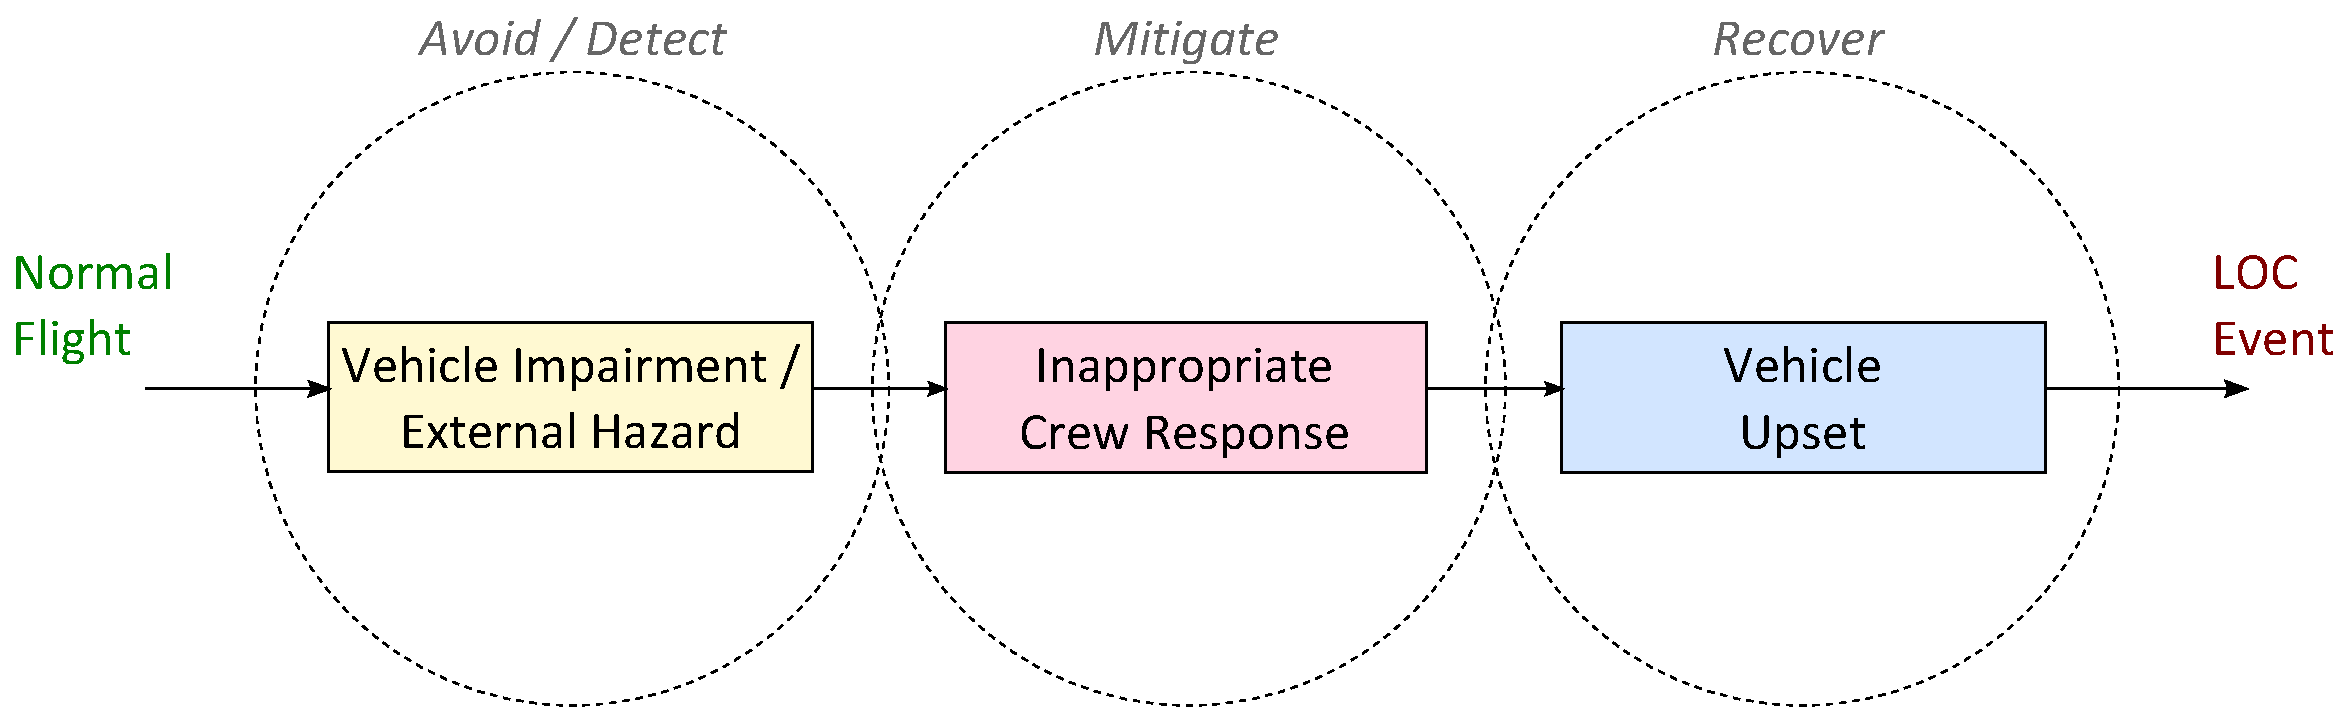
\includegraphics[width=0.60\textwidth]{LOC_accident_sequence.eps}
% 	\caption{\footnotesize Generic LOC sequence without onboard intervention technologies; figure adapted from~\cite{LOC10_Belcastro_concept}.}
%	\label{fig:gen_loc_sequence}
%\end{figure}
%-------------------------------------------------------------------------------------------------------


In the context of the AIRSAFE concept, we focus on the development of technologies that support the flight safety management and resilient control subsystem, and the onboard modeling capability. The proposed framework consists of four main components: a Resilient Flight Controller, a Flight Envelope Protection system with an LOC Prediction scheme, a Fault Detection and Isolation module, and a Flight Envelope Determination system. The four components work as an integrated system which is active throughout the entire flight. Hence, rather than intervening sequentially in an LOC chain, the system is constantly predicting the flight envelope and imminent LOC developments, and preventing and recovering from upset conditions.


%------------------------------------------------------------------------------
\subsection{Current Theoretical Developments and Results}
\label{subsec:current_develop}
%------------------------------------------------------------------------------

The research team has successfully completed extensive research in three key areas of this proposal: \emph{icing conditions of aircraft}, \emph{evaluation of pilot performance and error}, and \emph{robust adaptive flight control systems}. The proposed research will build further upon these results. Therefore, an overview of the results is presented in this section.

\subsubsection{Smart Icing Systems}

The ATR-72 accident in Roselawn,~IN, illustrates that ice accretion affects the performance and control of an aircraft and in extreme situations can lead to incidents and accidents. The Smart Icing Systems research program, funded by NASA~Glenn, conducted research at the University of Illinois on the development of a system to estimate aircraft performance and control changes due to ice, then use this information to automatically operate ice protection systems, provide aircraft envelope protection and, if icing was severe, adapt the flight controls~\cite{ICING_Bragg03}. This investigation was later used as a platform for continued development in systems-level icing protection system development~\cite{ICING_Gingras09}. As part of the Smart Icing Systems program, extensive  simulations for an aircraft in icing conditions were conducted to test the sensing and control adaptation techniques then under development~\cite{ICING_Bragg02}. These methods included the ability to scale the icing effects on the aircraft performance and control to various ice accretion flight and cloud conditions. These methods can be adapted to this research program. Additionally, a method for sensing ice-induced flowfield effects using aircraft control surfaces can also be integrated into the current research program to provide an additional source of sensing and predicting the effects of ice accretion on the aircraft performance and controllability. This method was initially developed as part of an FAA grant to better understand control degradation due to ice accretion~\cite{gurbacki}. Recently, further development of this method has provided improved sensing capability based on a better understanding of the iced wing flowfield and improved data analysis techniques~\cite{bragg2011_stall}.


\subsubsection{Evaluation of Pilot Performance and Error}

The human factors components of this project will require the development of quantitative and computational metrics and models of pilot error and the environmental and task conditions leading to error and other off-nominal control events. It will also require conducting pilot-in-the-loop experiments using flight simulation, and conducting statistical analysis and modeling of experimental data. In a series of research projects supported by NASA~Ames over the past 10~years, we have demonstrated an ability to diagnose sources of pilot error in both taxiing and approach-and-landing tasks using computational modeling~\cite{byrne2005aviation,byrne2007aviation}, an ability to diagnose, model and measure the factors that contribute to loss of situation awareness using statistical modeling techniques~\cite{kirlik2006situation}, and to verify these techniques using experimental methods~\cite{strauss2006situation}. In addition, and more recently, we have used the Beckman Institute flight simulator laboratory to conduct studies to develop and validate computational models and metrics of pilot performance and error in highly realistic scenarios drawn from actual historical data on operations at DFW~airport~\cite{zelma2011ACTR}. In this same simulation/experimental context, we have also created quantitative, entropy-based techniques that have been shown to be useful for predicting (human) controller failures to maintain on-time departure performance in DFW surface operations~\cite{moehlenbrink2012entropy}.


\subsubsection{$\Lone~$ Adaptive Flight Controller}

One of the critical components of the proposed framework for LOC prevention is the \emph{resilient flight control system}. The primary objective of this system is to provide predictable aircraft performance in the presence of uncertain dynamics, such as changes due to rapidly varying flight conditions during standard maneuvers and unexpected (moderate) failures. The design of the resilient flight controller for LOC prevention envisioned in this proposal builds on previous work by two members of the research team on $\Lone$~adaptive control~\cite{L1book}.

%In fact, adaptive control has long been seen as an appealing technology with the potential to prevent loss of control by improving aircraft performance in challenging flight conditions and by mitigating the impact of severe unexpected failures or vehicle damage. However, several deficiencies of the conventional adaptive algorithms have prevented these technologies from being widely used in safety-critical aerospace systems. $\Lone$~adaptive control overcomes these limitations and enables the design of predictable, repeatable, testable, and safe adaptive flight control architectures. The key feature of $\Lone$~adaptive control is the decoupling of the adaptation loop from the control loop, which enables \emph{fast adaptation} without sacrificing \emph{robustness}. Fast adaptation allows for compensation of the undesirable effects of rapidly varying uncertainties and significant changes in the system dynamics. In addition, fast adaptation is also critical to achieve predictable transient performance for system's both signals, input and output, without enforcing persistency of excitation or resorting to high-gain feedback.

The advantages of $\Lone$~adaptive control as a resilient flight control system were demonstrated in a series of remotely-piloted flight tests on the NASA AirSTAR Generic Transport Model~(GTM) aircraft, as part of the IRAC Project. The results from these flight tests showed that the $\Lone$~flight control law is able to provide predictable aircraft behavior under significant aerodynamic stability degradation as well as limited control authority, with a graceful performance reduction under increasingly severe adversity. The $\Lone$~control law also provided precision tracking capabilities with reduced pilot workload in stall and post-stall flight regimes, characterized by uncertain, unsteady, nonlinear phenomena. In addition, the $\Lone$~control law was used to support nonlinear unsteady aerodynamic modeling beyond the linear flight regime, and also enabled exploration of departure-prone edges of the flight envelope. In these modeling tasks, the $\Lone$~control law allowed the research pilot to operate the aircraft in precarious flight conditions near stall and in post-stall, and made the recovery post-departure more predictable and with lower workload. Flight test results for two of these modeling tasks are shown in Figure~\ref{fig:GTM.modeling}. Figure~\ref{fig:GTM.modeling.step} illustrates a precision tracking task in which the GTM was required to track a multistep wavetrain in the post-stall regime, while Figure~\ref{fig:GTM.modeling.schroeder} presents the response of the system to a Schroeder sweep, also in the post-stall regime. Further details about the design, performance, and flight tests of the $\Lone$~flight control law for the GTM aircraft can be found in~\cite{GNC09_AirSTAR,GNC10_AirSTAR,GNC11_AirSTAR,L1inflight}.


%--------------------------  FIGURE  ------------------------------------------
\begin{figure}[ht]
\centering
    \subfloat[Multistep command]{	 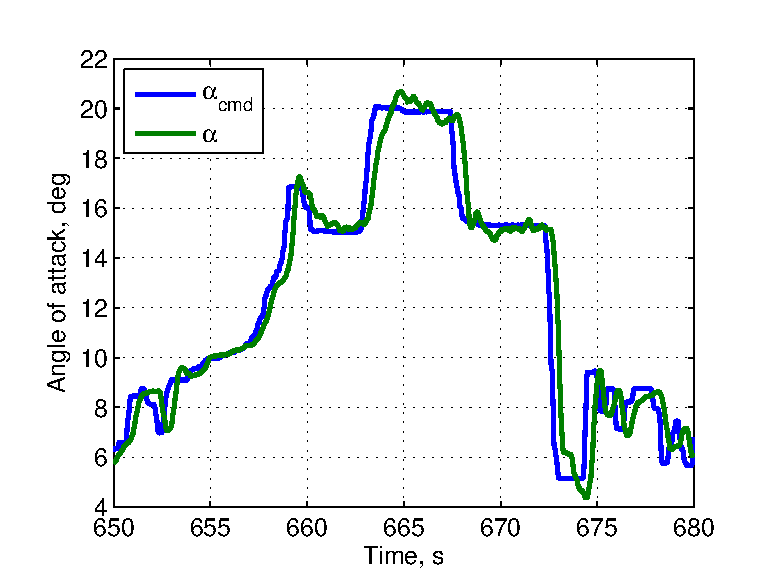
\includegraphics[width=0.35\textwidth]{AirSTAR/UnstdyAero_multistep.eps}\label{fig:GTM.modeling.step}
	}\hspace{5mm}
	\subfloat[Schroeder sweep]{
    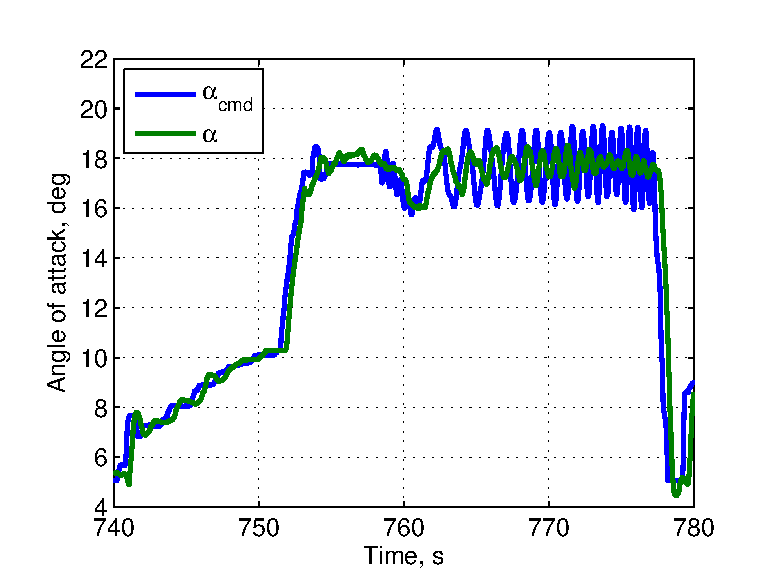
\includegraphics[width=0.35\textwidth]{AirSTAR/UnstdyAero_Schroeder.eps}\label{fig:GTM.modeling.schroeder}
	}
	\caption{\footnotesize $\Lone$~flight control law in support of unsteady aerodynamic modeling work in post-stall regimes.}
	\label{fig:GTM.modeling}
\end{figure}
%------------------------------------------------------------------------------


The series of flight tests on the GTM aircraft verified the theoretical predictions of the $\Lone$~flight control law, and also exposed some of its limitations. For instance, in the presence of a 125\%~stability degradation with an additional 50\%~reduction in pitch-control authority, the roll channel presented sustained oscillations and the aircraft started to exhibit PIO tendencies. These deficiencies were observed, for example, in the offset-to-landing task, the results of which are summarized in Table~\ref{table:CHRs}. As can be seen from the table, in the presence of a 125\%~stability degradation, the $\Lone$~control law --as designed-- was not able to ensure safe operation of the GTM~aircraft, which was flying at the verge of uncontrollability (CHR~7, Level~3 handling qualities). In this case, in order to ensure a predictable behavior of the impaired aircraft and prevent adverse pilot-aircraft coupling, it would have been necessary to \emph{reconfigure} the $\Lone$~flight control law based on information provided by an appropriately designed on-line fault detection and isolation algorithm.


%--------------------------  TABLE  -------------------------------------------
\begin{table}[h]
\centering
\scriptsize
    \caption{\footnotesize Summary of comments and CHRs from the offset-to-landing task; table taken from~[\citen{GNC11_GTMKevin}].}\label{table:CHRs}
    \renewcommand{\arraystretch}{1.1}
    \begin{tabular}{| c | c | c | c | c | c | c | c|}
    \hline\hline
    Flight \#    & Turbulence    & Stability     & Controllable? & Performance   & Workload      & Pilot             & CHR\\
                &               & Degradation   &               &               & tolerable?    & Compensation      & \\
    \hline\hline
                &               & Nominal       & Yes           & Desired       & Yes           & Minimal           & 3\\
    \cline{3-8}
    41          & Light         & 100\%         & Yes           & Adequate      & Yes           & Considerable      & 5\\
    \cline{3-8}
                &               & 125\%         & Yes           & Not           & Yes           & Max tolerable     & 7\\
                &               &               &               & adequate      &               & for performance   &\\
    \hline\hline
  	\end{tabular}
\end{table}
%------------------------------------------------------------------------------


%In this research effort, we will focus on the design of the reconfiguration logic for the $\Lone$-based resilient flight control system, and will integrate algorithms for fault detection and isolation, flight envelope determination and protection, and resilient control, giving special attention to LOC prediction and prevention. In the following sections we discuss the challenges and possible solutions for development and implementation of such technologies.



%------------------------------------------------------------------------------
\subsection{The Proposed Framework for LOC Prevention}
\label{subsec:framework}
%------------------------------------------------------------------------------

\subsubsection{Overview}

The integrated control architecture for aircraft resilience proposed in this research effort adopts the $\Lone$~flight control system introduced in the previous section, and augments it with algorithms and control schemes for fault detection and isolation, flight envelope determination and protection, as well as LOC prediction. Moreover, the proposed framework also extends the existing $\Lone$~flight control system so that both its control parameters and its structure can be reconfigured online based on the severity and nature of the identified failure. Next we present some details about the envisioned functionality of these elements and the reconfiguration logic for safe aircraft operation (see Figure~\ref{fig:RFTCarchitecture} for illustration):
\begin{itemize}
\setlength{\itemsep}{-1pt}
\vspace{-1mm}


\item \textbf{\emph{Resilient Flight Controller~(RFC)}:} The RFC is a high-performance flight control law designed to provide \emph{short-term stabilization} of the aircraft as well as \emph{improved maneuverability margins} at challenging flight conditions or in the event of moderate faults and failures. The RFC consists of two different modules: a \emph{baseline controller} and an $\Lone$~\emph{adaptive control augmentation}. The baseline controller is designed for a nominal aircraft model with the purpose of optimizing system performance, while the adaptive augmentation provides improved resilience by compensating for the undesirable effects of system uncertainty and unexpected disturbances.


\item \textbf{\emph{Flight Envelope Protection~(FEP)} and \emph{LOC Prediction}:} The FEP scheme ensures that the aircraft stays within its safe operational envelope by overriding, limiting, or shaping the commands generated by the pilot or the autopilot. The FEP is also designed to minimize adverse pilot-aircraft coupling and stops the pilot from making control inputs that would put the aircraft in a hazardous state. The FEP uses an \emph{LOC Prediction} module that uninterruptedly monitors the `position' of the aircraft within its flight envelope and, depending on the proximity to its boundaries, determines the `best' strategy to recover a safe operating condition. This block is thus crucial to prevent excursions outside the flight envelope that can lead to vehicle upsets and LOC events.


\item \textbf{\emph{Fault Detection and Isolation~(FDI)}:} The iReCoVeR system also implements an FDI algorithm, which runs in parallel to the RFC and is responsible for detecting and isolating adverse conditions such as sensor failures, vehicle impairment, or ice accretion. The FDI module uses the control signal generated by the RFC as well as the measured outputs to detect and isolate such adverse conditions. In the proposed framework, the RFC can be reconfigured on-line based on the information provided by this FDI module, which is critical to ensure a predictable behavior of the aircraft under severe faults or large changes in system dynamics.


\item \textbf{\emph{Flight Envelope Determination~(FED)}:} This block is responsible for determining an accurate estimate of the operational envelope of the possibly impaired aircraft. More specifically, this block relies on information provided by the FDI module described above as well as measured sensor data to establish safe limits for airspeed, angle of attack, angle of sideslip, pitch and bank angles, load factors, and control activity. The new estimate of the flight envelope generated by the FED is then sent to the FEP.

\end{itemize}


%--------------------------  FIGURE  ------------------------------------------
\begin{figure}[t]
\centering
\small
\psfrag{human}[lt][lc]{{\sf \it Pilot/Guidance Loops}}
\psfrag{irecover}[lt][lc]{{\sf \it LOC Prevention}}
\psfrag{aircraft}[lt][lc]{{\sf \it Aircraft}}
%
\psfrag{Situation}[cc][cc]{{\sf Situation}}
\psfrag{Awareness}[cc][cc]{{\sf Awareness}}
\psfrag{Interface}[cc][cc]{{\sf Interface}}
%
\psfrag{Safety}[cc][cc]{{\sf Safety}}
\psfrag{Monitoring}[cc][cc]{{\sf Monitoring}}
\psfrag{System}[cc][cc]{{\sf System}}
%
\psfrag{Pilot}[cc][cc]{{\sf Pilot}}
\psfrag{Autopilot}[cc][cc]{{\sf Autopilot}}
%
\psfrag{LOC}[cc][cc]{{\sf LOC}}
\psfrag{Prediction}[cc][cc]{{\sf Prediction}}
%
\psfrag{Stability}[cc][cc]{{\sf Flight}}
\psfrag{Envelope}[cc][cc]{{\sf Envelope}}
\psfrag{Protection}[cc][cc]{{\sf Protection}}
\psfrag{Determ}[cc][cc]{{\sf Determination}}
%
\psfrag{FDI}[cc][cc]{{\sf FDI}}
\psfrag{Module}[cc][cc]{{\sf Module}}
%
\psfrag{RFC}[lc][lc]{{\sf Resilient Flight Control}}
\psfrag{L1}[cc][cc]{{\sf $\Lone$ Adaptive}}
\psfrag{Aug}[cc][cc]{{\sf Augmentation}}
\psfrag{Baseline}[cc][cc]{{\sf Baseline}}
\psfrag{Controller}[cc][cc]{{\sf Controller}}
%
\psfrag{RFTC}[rc][rc]{{\sf iReCoVeR}}
%
\psfrag{Aircraft}[cc][cc]{{\sf Aircraft}}
\psfrag{Sensing}[cc][cc]{{\sf Sensors}}
%
\psfrag{fdi}[lc][lc]{{\sf \it FDI}}
\psfrag{trigger}[lc][lc]{{\sf \it trigger}}
%
\psfrag{reconf}[lc][lc]{{\sf \it reconfig.}}
%
\psfrag{situation}[lc][lc]{{\sf \it Situation}}
\psfrag{awareness}[lc][lc]{{\sf \it Awareness}}
%
\psfrag{r}[cc][cc]{$r$}
\psfrag{u}[cc][cc]{$u$}
\psfrag{y}[cc][cc]{$y$}
\psfrag{yh}[cc][cc]{$\hat{y}$}
%
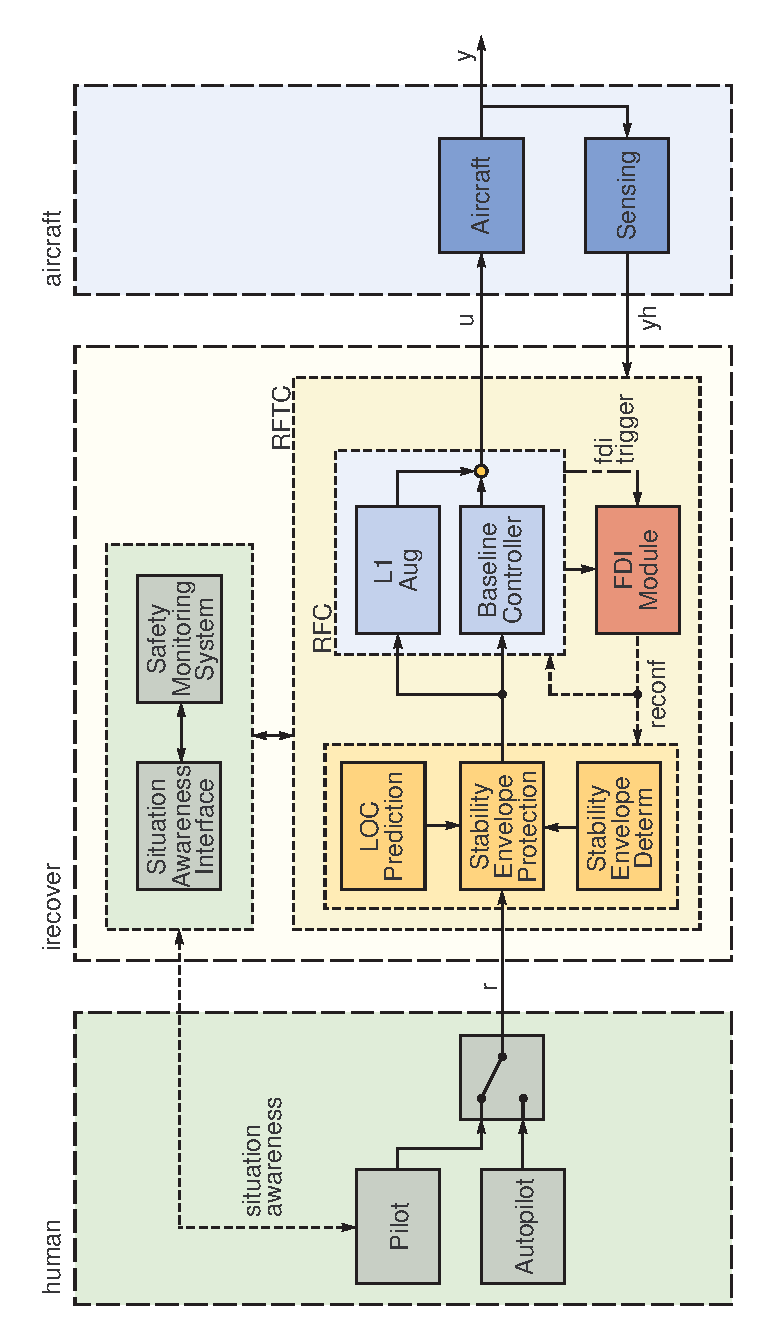
\includegraphics[angle=-90,width=0.90\textwidth,]{RFTCarchitecture.ps}
\caption{\footnotesize A flight control architecture for loss-of-control prevention (simplified).}
\label{fig:RFTCarchitecture}
\end{figure}
%------------------------------------------------------------------------------


%%At this point, it is important to note that, in order to ensure safe and effective pilot-automation interaction, the crew must be kept maximally informed about the state of the iReCoVeR system as well as its current and expected behaviors~\cite{kirlik2006situation}. This is why, in the envisioned framework, the status of both the aircraft and the iReCoVeR system are being continuously monitored by the \textbf{\emph{safety monitoring system}}, which analyzes the time-evolution of signals that are critical to ensure safe operation of the aircraft, such as the outcome of the FDI and the LOC prediction modules. The safety monitoring system is also responsible for selecting and elaborating the most relevant information to be provided to the crew. This information is then sent to the \textbf{\emph{situation awareness interface}}, which provides visual, auditory, and possibly tactile feedback to the pilot. The purpose of this interface is to make the automation's compensation transparent to the crew, ensuring safe and effective pilot-automation interaction. Moreover, the safety monitoring system and the situation awareness interface are to be designed and evaluated so that the information provided --as well as its representation-- does not lead to an unacceptable increase in pilot workload. Although the design of a safety monitoring system and a situation awareness interface is \underline{not} an integral part of the proposed research, the verification and validation of the developed iReCoVeR system needs to take these (human) factors into account to properly asses the efficiency of automation.
%
%\medskip

In the following subsections we discuss some of the challenges and possible solutions for design and implementation of this technology.


\subsubsection{Resilient Flight Controller}

As demonstrated in the AirSTAR flight tests, the $\Lone$-based RFC is able to compensate for system uncertainties and faults, and provide a predictable aircraft behavior, with a graceful performance degradation under increasing adversity. Moreover, in the case of severe failure, the $\Lone$-based RFC is also able to prolong the critical time window\footnote{The expression `critical time window' is defined in~\cite{LOC04_LOCMetrics} as the ``interval between the time of the first envelope excursion and the time when control was lost''.}; this is of particular interest in the present framework, in which this extra time might be critical to ensure that the FDI algorithm can effectively detect and isolate the adverse condition, before it evolves into a full-blown hazardous scenario.


One of the limitations of the $\Lone$~flight control laws designed so far is that they are \emph{passive}, meaning that the impaired aircraft continues to operate with the same flight control law. One of the objectives of the proposed research is to put forward an \emph{active} $\Lone$-based RFC that is reconfigured based on the information provided by the FDI module. This poses several challenges. First, a \emph{reconfiguration logic} must be included in the control system that guarantees a safe transition from the old configuration to the new one, while yet ensuring a prompt recovery of the aircraft. In particular, this logic should try to minimize undesirable transients that can potentially lead to an adverse pilot-aircraft interaction or to structural loads that exceed the design strength of the airframe components. And second, depending on the severity of the failure, the remaining control authority might be significantly reduced --placing undesirable limits on the maneuverability of the aircraft-- or might not even be sufficient to stabilize the aircraft. In these scenarios, the use of \emph{unconventional control configurations} might be required or highly desirable. Therefore, we will $(i)$~develop algorithms for safe control reconfiguration and characterize their transient behavior; $(ii)$~determine off-nominal scenarios that require the use of unconventional control configurations; and $(iii)$~develop adaptive control allocation schemes with guaranteed stability and performance characteristics.



\subsubsection{Flight Envelope Protection and LOC Prediction}

The proposed FEP scheme considers the five operational envelopes identified in~\cite{LOC04_LOCMetrics}, which account for adverse aerodynamic excursions, unusual attitudes, structural integrity, and control authority (see Figure~\ref{fig:LOCenvelopes}). As described in~\cite{LOC04_LOCMetrics}, an excursion that goes outside (at least) three of these envelopes is a clear indication of LOC, while standard operational maneuvers usually do not lead to an excursion outside more than one envelope. The goal of the FEP is thus to correct the pilot (or autopilot) control inputs to ensure that the aircraft stays within its safe operational envelopes. For this purpose, the \emph{LOC Prediction} module monitors the `position' of the aircraft within these envelopes and, depending on the proximity to the boundaries, determines the `best' strategy to maintain the aircraft within its envelopes or, in case of aircraft upset or imminent LOC~event, to recover a safe flight condition.


%--------------------------  FIGURE  ------------------------------------------
\begin{figure}[ht]
\centering
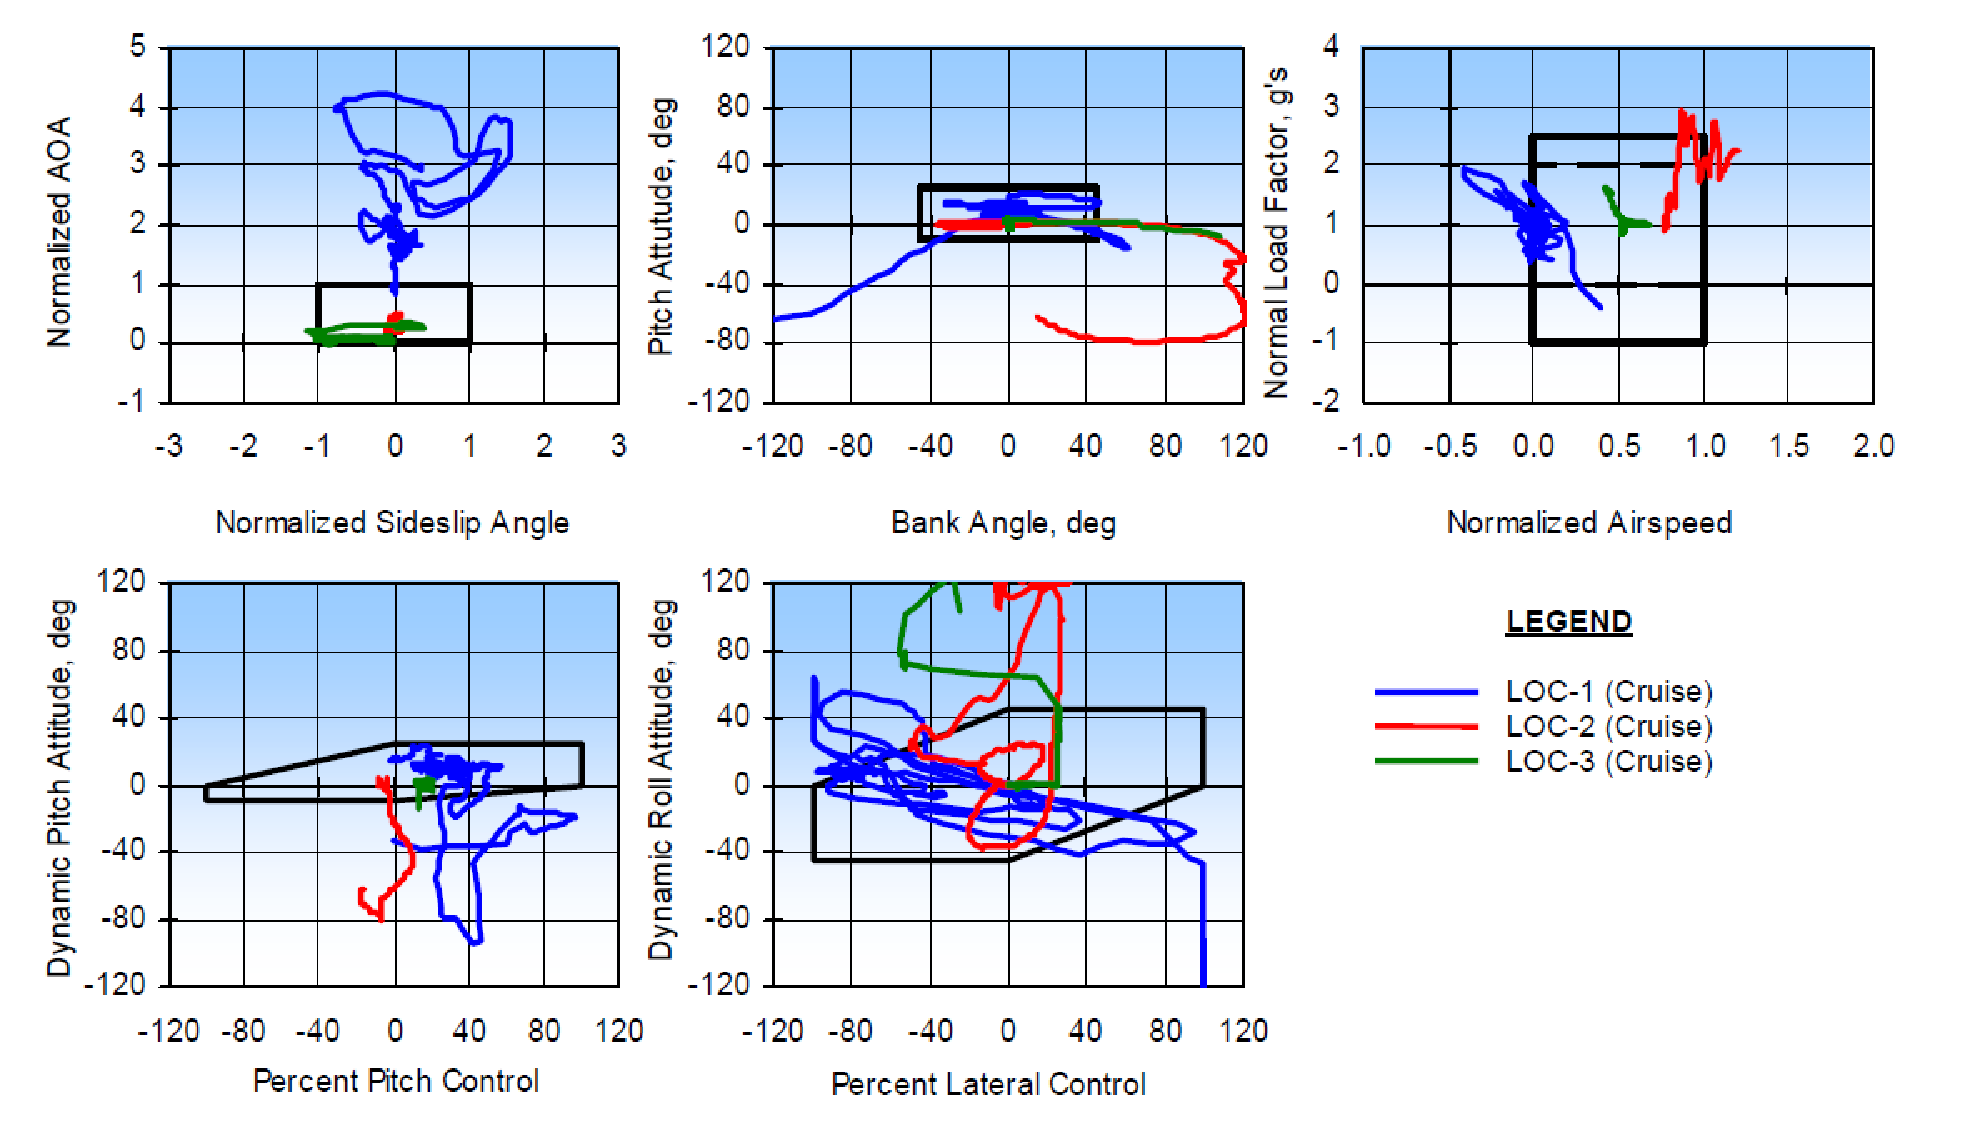
\includegraphics[width=0.65\textwidth,]{LOCenvelopes.eps}
\caption{\footnotesize LOC excursions exceeding the operational flight envelopes; figure taken from~\cite{LOC04_LOCMetrics}.}
\label{fig:LOCenvelopes}
\vspace{2mm}
\end{figure}
%------------------------------------------------------------------------------


In this research effort, we intend to investigate two different strategies for flight envelope protection. The first one relies on the implementation of a model predictive controller~(MPC), which is well-known for approximately solving constrained optimal control problems~\cite{aut00_MPC}. MPC is able to accommodate hard constraints on both control inputs and system states, which makes it particularly interesting in the application at hand. There are several challenges in applying MPC to uncertain systems. First, system uncertainties can severely affect system stability and performance. Traditional robust MPC approaches consider bounded, state-independent uncertainties, and provide worst-case solutions by solving a ${\min}$-${\max}$ problem. However, in our case, the uncertainty present in the system is state-dependent. In this context, it seems MPC can benefit from the presence of the $\Lone$~control augmentation in the RFC, which is able to estimate and compensate for the uncertainties present in the system and provide a consistent aircraft behavior. Research will investigate this $\Lone$-MPC approach, and will establish stability and performance guarantees as well as systematic methodologies for the design of model predictive controllers for uncertain systems.


The second strategy for flight envelope protection is to extend the $\Lone$~adaptive control theory to cope with nonlinear systems that need to operate within given input and/or output constraints. Preliminary theoretical results of this extension can be found in~\cite{Infotech11_L1constraints}, while the application of this preliminary approach to aircraft engine control is presented in~\cite{Infotech11_L1engine}. The current theoretical framework, however, is limited to single-input single-output plants with only matched uncertainties. The proposed research will address these issues and will try to put forward an adaptive control scheme that can handle multiple-input multiple-output systems in the presence of general unmatched uncertainties, while simultaneously satisfying input and output constraints.



\subsubsection{Fault Detection and Isolation and Control Reconfiguration}

Detection and isolation of adverse conditions is a crucial step in iReCoVeR. The FDI module is expected to detect and isolate an adverse condition, while at the same time identifying a model of the impaired aircraft. As mentioned earlier, the proposed framework will accommodate system failures, vehicle impairment, and changes in aircraft dynamics due to ice accretion. Also, note that, the FDI module is not in the critical path (see Figure~\ref{fig:RFTCarchitecture}) and is only used to reconfigure other elements of iReCoVeR, such as the RFC and the FEP systems.


In general, FDI methods take advantage of the concept of redundancy, which can be classified as either \emph{hardware redundancy} or \emph{analytical redundancy}. On one hand, hardware redundancy consists of monitoring duplicative signals generated by different devices and comparing these signals using various methods~\cite{nelson1968cross,hfling1995observer}. On the other hand, analytical redundancy uses mathematical models together with estimation tools, including observer-based methods~\cite{patton1991robust,patton2000eigenstructure,beard1971failure,white1987detection,park1994new,park1994new2,douglas1999h}, unknown input observer approaches~\cite{watanabe1982instrument,wunnenberg1987sensor,frank1989robust,chen1996design,demetriou2005using,hou1992design}, parity relations approaches~\cite{gertler1997fault,patton1991robust,patton1994review,chan2006application}.  Surveys on analytical redundancy can be found in~\cite{gertler1988survey,frank1990fault,frank1997survey,hwang2010survey}.


In the proposed framework, we consider an analytical redundancy approach based on multiple-model FDI methods~\cite{cdc99_MMFDI,tcst08_MMFDI}. The basic idea is to use the control signal that is applied to the actual aircraft to run a set of off-nominal aircraft models. The outputs of these models are then compared (over a finite-time running window) to the measured output of the aircraft, and the model showing the smallest residuals is identified as the ``closest'' model to the current aircraft configuration. In order to improve the accuracy and reliability of the isolation process, this multi-model FDI algorithm will be augmented with other FDI approaches such as on-line aerodynamic parameter estimation~\cite{gnc09_FEEP,AFM10_MorelliEstimation}. This FDI module can also receive and accommodate information from other \emph{health management systems} implemented onboard the aircraft.


%--------------------------  FIGURE  ------------------------------------------
\begin{wrapfigure}{r}{0.4\textwidth}
\centering
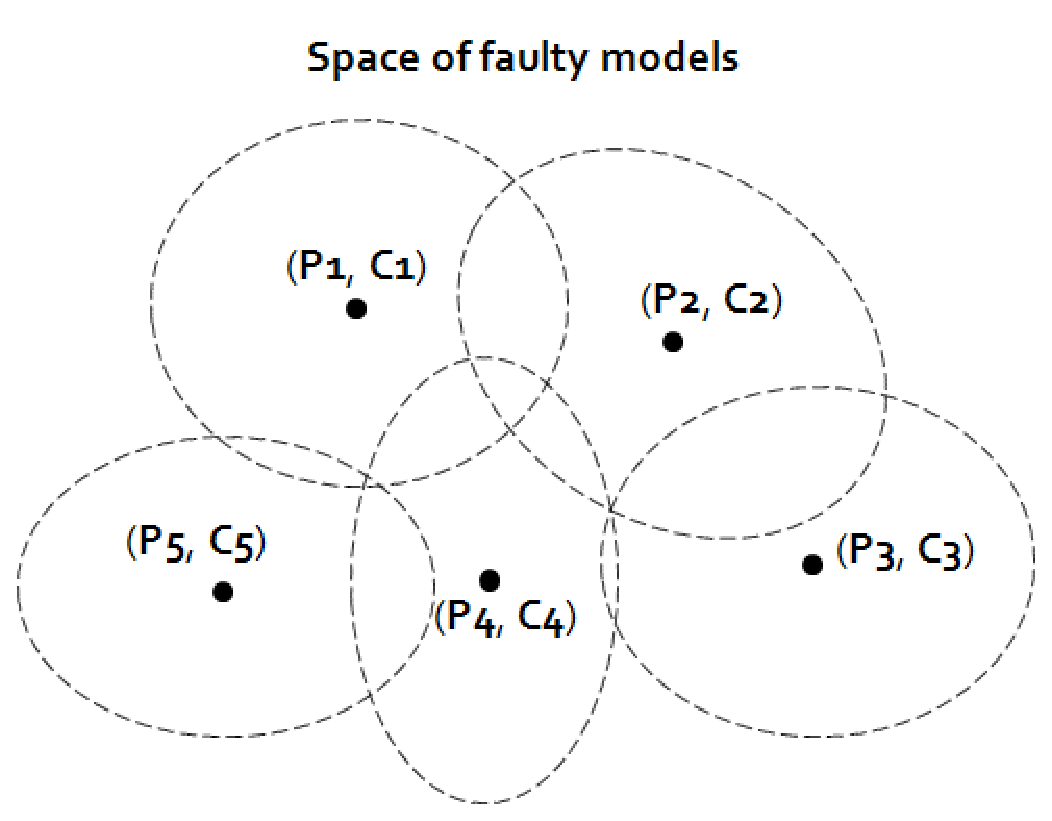
\includegraphics[width=2.3in]{FDImodes.eps}
\caption{\footnotesize Adverse-condition coverage.}
\label{fig:FDImodes}
\end{wrapfigure}
%------------------------------------------------------------------------------


A first essential question that needs to be addressed is the choice of the number and nature of off-nominal models needed to accurately isolate the adverse condition. Obviously, it is impractical to list all possible adverse conditions. Meanwhile, we know that $\Lone$~adaptation is able to compensate for certain level of uncertainties. Therefore, to some extent, we can use adaptation to compensate for the mismatch between the mathematical models in the FDI library and the actual faulty aircraft. Consequently, the selection of off-nominal models is coupled with the compensation ability of the $\Lone$~adaptive controllers. To illustrate this, let $\mathcal{M}$ be the set of models in the library. Each model ${\bf P}\in\mathcal{M}$ is associated with an $\Lone$-based RFC, denoted by ${\bf C}$. Then we know that a class of off-nominal models can be covered by the pair~$({\bf P, C})$, in a sense that if the mismatch between the actual aircraft and the model~${\bf P}$ is within certain bounds, then ${\bf C}$ can ensure stability and desired performance. Let $\mathcal{W}$ be the set of all controllers~${\bf C}$. We now discuss our approach towards the choice and design of off-nominal models in~$\mathcal{M}$ and RFCs in~$\mathcal{W}$. The main idea can be summarized as follows: first, we sample the off-nominal models and make sure that the mismatch between two neighboring models is within an acceptable ``range''; and second, for each sampled model, we design an RFC that is able to accommodate the mismatch between neighboring models (see Figure~\ref{fig:FDImodes}). It is clear that, while a large number of pairs~$({\bf P,C})$ leads to enhanced aircraft performance in the presence of adverse conditions, such a solution would also increase the complexity of the iReCoVeR system and thus lead to higher verification costs. Therefore, one of the objectives of the proposed research is the design of strategies to solve this trade-off. A second question that needs to be addressed is the quantification of the runtime required for the FDI module to converge and isolate an off-nominal model. For this purpose, we will rely on Lyapnuov approaches~\cite{Seto96,cervin02,bamieh03,marti04,nesic-04,palopoli-05,imer2006measure,tabuada2007tac,cervin2008scheduling,mmazo2008cdc,pwan2009cdc, heemels2010tac}.


We also note that the $\Lone$-based RFC can be used to monitor the status of the aircraft and the automation itself, and can help detect adverse conditions. In particular, there are three signals that are of special interest: $(i)$~the filtered estimate of the uncertainty generated by the $\Lone$~adaptation law; $(ii)$~the difference between the output of the aircraft and the output of the $\Lone$~predictor; and $(iii)$~the difference between the output of the aircraft and the output of a pre-specified ideal (reference) model. Under nominal operating conditions, these three signals should be ``small'', indicating that the current aircraft model used in the RFC correctly represents the actual aircraft dynamics and that the RFC is providing close-to-desired performance. On the other hand, a ``large size'' of any of these three signals would indicate that the aircraft is experiencing an off-nominal condition. %For instance, if the uncertainty estimate were ``large'', then it would mean that there is a significant mismatch between the aircraft model used in the RFC and the actual aircraft dynamics, which would point in turn to the existence of an adverse condition. % Also, a ``large'' difference between the aircraft output and the ideal-model output would indicate the infeasibility of the current control objective and the necessity of reconfiguring the RFC.
It is also important to emphasize that the parameter estimates of the adaptive algorithm (similar to the estimates of other on-line identification schemes) have to be used cautiously for control purposes, as parameter convergence is \underline{not} guaranteed in general.

\medskip

Next we present details of two specific areas that will be considered in this research effort: \emph{in-flight aircraft icing} and \emph{sensor failures}.

\paragraph{In-Flight Aircraft Icing:} We propose two primary tasks to better understand the effect of ice accretion on aircraft performance and control, and to provide representative iced aircraft stability and control models:
\begin{itemize}
\setlength{\itemsep}{-2pt}
\vspace{-2mm}

\item Develop performance and control models, based on existing steady-state data and methods. We will develop two primary models for this task. The first will be a symmetric model where the ice accretion is symmetric about the aircraft $\mathit{xz}$-plane of symmetry.  This model will be developed to allow it to be scaled for icing conditions of various intensities using the techniques outlined in~\cite{ICING_Bragg02}. The second model will be the asymmetric model where the ice accretion is assumed to be asymmetric with respect to the aircraft $\mathit{xz}$-plane. This model will also be developed to enable scaling of the icing conditions and severity of the performance and control degradation. %Asymmetric icing encounters, like that seen by the ATR-72 accident aircraft, are especially hazardous and are particularly susceptible to rapid roll and departure as stall is approached.


\item Icing accidents usually occur in highly dynamic environments where flow separation and rapid movement of control surfaces lead to highly unsteady separated flows that are not currently considered when developing iced aircraft models. To extend the state-of-the-art in iced aircraft modeling, we propose to develop extensions to the above models that include unsteady aerodynamics effects, particularly those coupled to the rapid movement of the wing and tail control surfaces. The proposed research would experimentally investigate the coupled effects of aircraft icing and dynamic control-surface deflection on the unsteady flowfield around an airfoil under conditions similar to aircraft approach and landing. Using these data, we would modify the steady-state model to better include these unsteady effects and better simulate accident-like scenarios in icing.

\end{itemize}


\paragraph{Sensor Failures:} Sensor failure is an important class of hardware failure that poses several challenges to detection and control schemes~\cite{willsky1976survey,akyildiz2002survey}. Since sensors provide feedback signals to the control algorithms, any malfunction of the sensing process will directly affect the performance capabilities of the control laws. In addition, most controllers are not able to detect such failures. Therefore, in order to ensure a safe aircraft operation, sensor failures need to be handled through systematic methods involving detection, isolation, and mitigation~\cite{naidu1990use,guo1991sensor,napolitano1995neural}. In this research effort, we will explore the application of analytical redundancy approaches~\cite{randell1975system,chow1984analytical,ammann1988data,eckhardt1991experimental,maybeck1999multiple}, as well as the implementation of adaptive estimation schemes to identify and isolate structured sensor failures (e.g. additive or multiplicative measurement errors). Other techniques such as Kalman filtering~\cite{welch1995introduction} or the support vector machine~\cite{suykens1999least} will also be explored. The information provided by these detection and isolation schemes will then be used to ensure safe operation of the aircraft despite the sensor failure. On one hand, if the failure is successfully isolated, the measurement can be corrected before being used in the control laws. On the other hand, if the failure is detected but not perfectly isolated, then the RFC and the FEP scheme might need to be reconfigured to a high-assurance low-performance control mode with reduced sensitivity to sensor data.



\subsubsection{Flight Envelope Determination}

In the proposed framework, the FED scheme, responsible for determining an estimate of the operational envelope of the possibly impaired aircraft, relies on a library of pre-computed safe flight envelopes. In the setup adopted, these envelopes correspond to the off-nominal models used in the FDI module and, therefore, once the adverse condition has been isolated, the flight envelope for the identified aircraft model can be easily estimated by simple interpolation of the envelopes stored in the library. This approach is computationally efficient and provides reasonably accurate estimates of the operational envelopes, provided the FDI is able to reliably isolate the adverse condition.



%------------------------------------------------------------------------------
\subsection{Verification and Validation}
%------------------------------------------------------------------------------

In order to validate the effectiveness and performance of the proposed research in preventing LOC, the iReCoVeR system will be implemented in the Human-in-the-Loop~(HITL) flight simulation facility at the University of Illinois's Beckman Institute. The team also proposes to transition the developed LOC prevention framework to NASA LaRC for implementation on the AirSTAR flight test facility, which provides an actual flight environment to validate the developed technologies.


\subsubsection{Full-Scale Aircraft Human-in-the-Loop Experiments}

As an integral part of the proposed research, we will use a medium-fidelity flight simulator to test, refine, and ultimately verify our approach to prevent LOC under adverse conditions and pilot input errors. To do so, we will use a HITL flight simulation facility at the University of Illinois that a member of the research team is currently using to conduct NASA-sponsored human factors NextGen aviation research.


%--------------------------  FIGURE  ------------------------------------------
\begin{wrapfigure}{r}{0.64\textwidth}
\centering
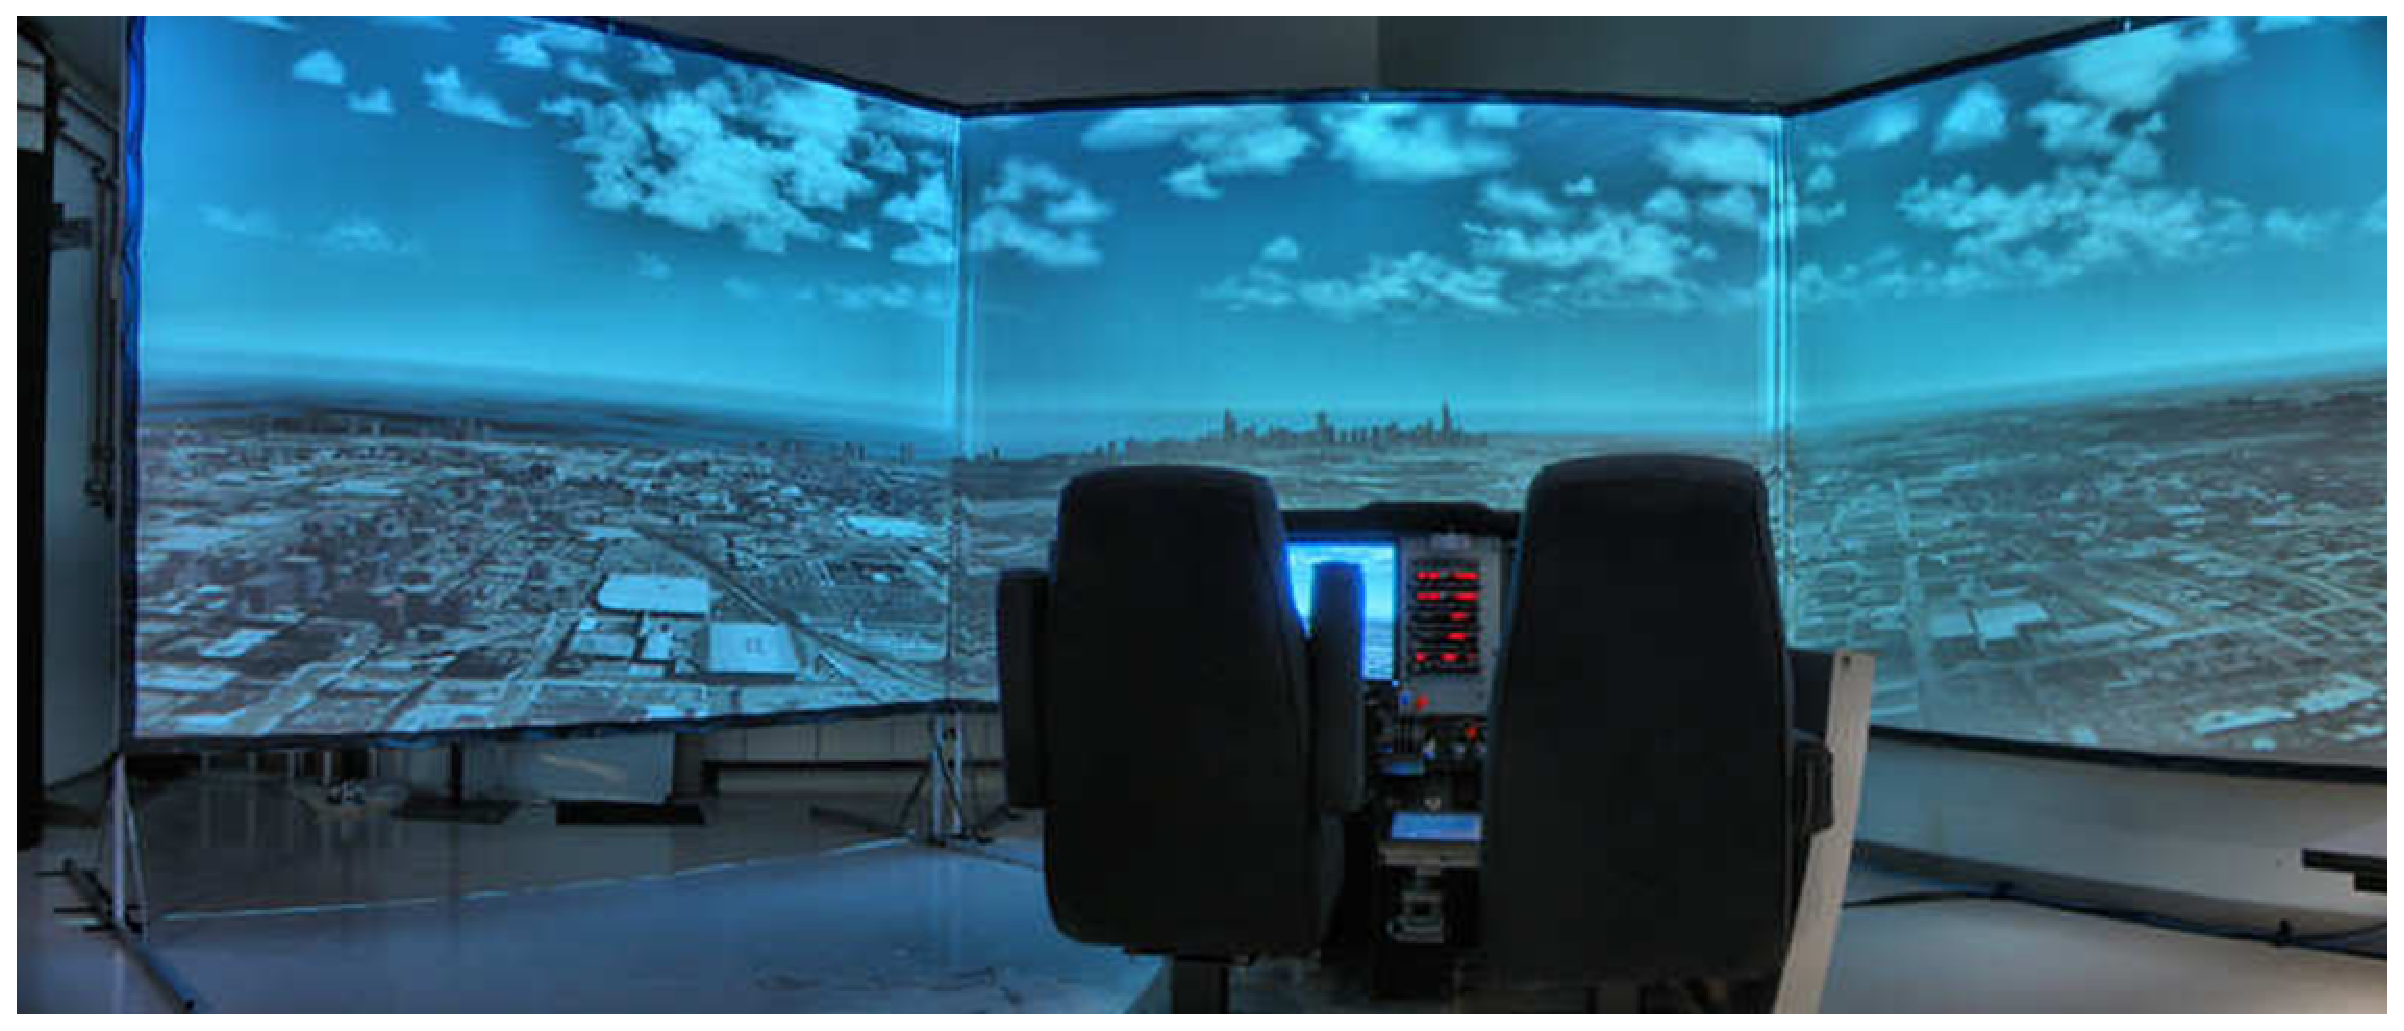
\includegraphics[width=0.64\textwidth]{simulator.eps}
\caption{\footnotesize The Beckman Institute Flight Simulator at UIUC.}
\label{fig:simulator}
\end{wrapfigure}
%------------------------------------------------------------------------------


The HITL flight simulation facility at the University of Illinois's Beckman Institute (shown in Figure~\ref{fig:simulator}) has recently been upgraded to support the use of X-Plane~9.40 and is outfitted with state-of-the-art eye-tracking technology. The flight simulator hardware is based on a Frasca~142 simulator cockpit that has been upgraded so that all cockpit information displays can be reconfigured via software. Graphics are provided by a cluster of PCs, allowing for the easy addition of heads-up, heads-down, and lateral displays. The current version of X-Plane provides an experimental design palette, which includes 867~instruments, 25,737~airports, 25,866~Navaids, 88,367~fixes, and 18,008~scenery files. This scenery is of reasonably high fidelity, as depicted in Figure~\ref{fig:simulator}.


For the experiments, control input errors to be considered are those likely to result from spatial disorientation and/or loss-of-energy state awareness by the pilot. Neither of these control error conditions preclude the possibility of manual reversion from autopilot control as a precursor event. Therefore, we intend to ascertain those flight situations that are most likely to produce loss of control, both with and without an autopilot induced manual reversion event. It is also important to consider situational awareness, with or without ensuing spatial disorientation, as an important precursor event to an induced loss of control. In this latter case, we believe those tasks or flight conditions that lead to loss of situational awareness, while at the same time an externally produced departure from steady-state control occurs, are potentially good candidates for setting up the pilot for an LOC event. Sensor deficiencies or failures and other external disturbances, such as icing or turbulence, will also be examined to determine the likelihood of inducing pilot control errors which directly or indirectly lead to LOC events within our simulation environment. In determining the best candidate maneuvers or flight situations in which to induce an LOC event, as a result of one or more of the previously mentioned crew errors or adverse conditions, we will perform a literature and accident report review, as well as perform a preliminary study with pilot participants. In general, this preliminary work is necessary in order to determine the level of steady-state flight perturbations that produce an LOC event severe enough to see the benefits of iReCoVeR.


Additionally, crew performance metrics will be developed in order to quantify the nature and magnitude of pilot errors leading to an LOC, as well as performance during recovery with and without iReCoVeR. Metrics that address both the time to recovery and accuracy of pilot control input during recovery will be developed and validated during the preliminary phase of the project.


\subsubsection{Technology Transition to NASA and Flight Tests of AirSTAR Testbed}

We propose to transition the developed framework to the facilities of NASA LaRC, and in particular to the NASA AirSTAR GTM testbed. The AirSTAR flight test facility would allow us to validate the developed work against flight environment conditions with a pilot in the loop. The team has collaborated extensively with researchers from NASA LaRC for the IRAC Project and is familiar with the Generic Transport Model and the hardware infrastructure. Therefore, it is expected that implementation and debugging efforts will be reduced significantly, which ensures a smooth transfer of the developed technologies to the AirSTAR flight test facility.





%==============================================================================
\section{Impact and Relevance of the Proposed Research}
%==============================================================================

$\Lone$ adaptive control is a part of the Aviation Safety Program. It was initially introduced in the IRAC Project of 2007-2010 and can serve as an enabling technology for other tools in the VSST successor project. It is also being considered in the Fundamental Aeronautics Program, Fixed Wing Project. The objective here is to control very flexible vehicles, thus enabling significant weight reduction which leads to better fuel efficiency. Discussions are ongoing for applying $\Lone$~adaptive control to studies for Space Exploration related applications (such as the next generation launch vehicles and planetary exploration concepts) and to rapid prototyping of innovative UAV concepts at NASA LaRC. We hope that, given both the opportunity to contribute to these programs and appropriate levels of funding, the solutions proposed by us can be matured and transitioned to NASA LaRC and support NASA LaRC in holding a leadership role in the Aviation Safety Program.

Growing overseas interest in $\Lone$~adaptive control comes from our European partners in The Netherlands (Delft University of Technology, TUD) and Germany (Technical University of Munich, TUM), who are exploring new aerospace platforms to implement $\Lone$~adaptive control. At TUD an $\Lone$~adaptive flight controller has been designed for the Citation~II business jet, a state-of-the-art flying laboratory of the university. Handling qualities experiments have been conducted on the SIMONA, a 6-DoF, motion-based research flight simulator, to assess the performance of the $\Lone$~flight controller in the presence of anomalies~\cite{GNC11_L1Citation}. The aim is to transition the $\Lone$~adaptive flight controller to the Citation~II and conduct piloted flight tests. Several projects are in the works at TUM. An $\Lone$~adaptive control augmentation for an NDI~autopilot is being developed for the MBDA Generic Missile~\cite{GNC12_L1missileTUM}. $\Lone$~adaptive flight controllers are also being designed for and implemented on a Hummingbird Quadrotor and a DA-42 twin seat, propeller-driven aircraft, operated by TUM. The latter is another effort to transition $\Lone$~adaptive control to manned aircraft.

%It is important to note that $\Lone$ adaptive control is also being widely applied to areas other than aeronautics, \cite{ZLi09ACC,ZLi09GNC,ZLi10CDC,ZLi11MSC_Drilling,Sun11MSC_Rotary,Carolyn2011acc}. Besides DoD programs and applications to autonomous systems, we have obtained funding from Seagate for disk drive control, from StatOil for drilling applications in oil production, from Raymarine for autopilot design for various classes of boats. Our collaborators have explored applications in anesthesia using clinical data. Lastly, we are looking into human-robotic space applications as part of a NASA SBIR program with CU Aerospace, LLC.



%==============================================================================
\section{General Plan of Work}
%==============================================================================

%------------------------------------------------------------------------------
\subsection{Key Milestones}
%------------------------------------------------------------------------------

Within the next thirty-six months, if funded, the team of co-Is of this proposal will be working on the development of iReCoVeR. We hope that in the third year we will conduct an intensive evaluation of iReCoVeR in the flight simulator facility of the Beckman Institute at UIUC. We propose the following schedule with the understanding that the time frames for these milestones can be refined based on our interaction with NASA LaRC.

\begin{description}

  \item[Year I:] ~(FDI, RFC)~  We will work on synthesizing the iReCoVeR architecture and integrating it in the flight simulator of the Beckman Institute. Some of the blocks of iReCoVeR will be in passive mode and will be activated within the subsequent years.
         \begin{enumerate}
         \vspace{-2mm}
         \setlength{\itemsep}{-1pt}

          \item Bragg will work on the development of the symmetric and asymmetric ice accretion models, based on existing steady-state data and methods. In parallel, he will start working on the design of wind-tunnel experiments to study the unsteady aerodynamic effects due to the interaction of icing with control-surface movements.

          \item Kirlik will perform a literature and accident report review, as well as a preliminary study with pilot participants, to determine the best candidate maneuvers or flight situations to induce LOC events. Based on this study, his team will design scenarios that reliably lead to pilot-induced LOC events, and program the flight simulator to embed the required design features. He will also develop a set of metrics to characterize pilot-induced LOC events. Additionally, Kirlik will collaborate with Bragg on the integration of the icing models in the simulator.

          \item Cao will develop sensor failure modes and will collaborate with Hovakimyan on the development of the FDI module and the safe control reconfiguration mechanism of the $\Lone$-based RFC. They will identify the off-nominal scenarios that require the use of unconventional control configurations. They will also develop adaptive control allocation schemes with guaranteed stability and performance characteristics. By the end of the first year, the team hopes to deliver a prototype of an \emph{active} $\Lone$-based RFC.

          \item Hovakimyan will collaborate with  Kirlik on the integration of the corresponding solutions into the flight simulator. The team hopes to have a prototype of the FDI and RFC modules functioning in the flight simulator within the first year.

        \end{enumerate}



    \item[Year II:] ~(FEP, FED)~ We will focus on the development of the FEP and FED schemes as well as the required modifications to the RFC.
        \begin{enumerate}
         \vspace{-2mm}
         \setlength{\itemsep}{-1pt}

            \item Hovakimyan and Cao will work on the development of the FEP and LOC prediction modules. An algorithm will be developed to monitor the proximity of the aircraft to the boundaries of the five operational flight envelopes for LOC prediction. They will also explore the feasibility of the two proposed strategies for FEP described in this proposal, and will develop theoretical guarantees for the most suitable method.

           \item Hovakimyan will work with Cao and Bragg on the development of the FED module, by creating a library of pre-computed flight envelopes in full coordination with NASA.

            \item Bragg will conduct wind-tunnel tests to extend the steady-state icing models to include unsteady effects due to the interaction of icing with control-surface movements.

            \item Kirlik will perform intermediate human-in-the-loop evaluations of the developed RFC and FDI modules on the simulator. He will also develop a set of safety-assessment metrics for pilot errors or off-nominal behaviors and program any necessary simulator autopilot interface to delimit the range of pilot inputs (if necessary). In parallel, Kirlik will work with Hovakimyan and Bragg on the integration of the corresponding solutions and icing models into the flight simulator.

        \end{enumerate}

      \item[Year III:] ~(iReCoVeR)~ We will work on intensive validation of the iReCoVeR system in the flight simulator of the Beckman Institute and transitioning of iReCoVeR to NASA AirSTAR. We will also collaborate with NASA researchers on the flight tests of the AirSTAR testbed.
        \begin{enumerate}
         \vspace{-2mm}
         \setlength{\itemsep}{-1pt}

            \item Kirlik will conduct experimental evaluations of the proposed iReCoVeR system using proper experimental controls and skilled pilot participants. He will also analyze the results of these evaluations using safety-assessment metrics based on both summary and inferential statistics (ANOVA) to determine the efficacy of iReCoVeR.

            \item Hovakimyan and Cao will transition the iReCoVeR system to NASA AirSTAR and support both the developments and flight tests.

            \item Bragg will assist NASA AirSTAR in developing ice accretion models for their high-fidelity simulation environment.

            \item All four members of the team will cooperate on the refinement of iReCoVeR based on pilot feedback, and will finalize the first release of iReCoVeR to NASA. The team expects that over the years iReCoVeR will be used on other platforms at NASA.

        \end{enumerate}

    \item[Reporting:] It is anticipated that reporting of results will be done to NASA on an as-needed basis. Further, a yearly progress report will be filed, as well as an end-of-project report detailing all the findings. Results will also be published in conferences and archival journals.

\end{description}


\subsection{Management Structure}
Naira Hovakimyan will be the PI on this proposal. She will closely collaborate with Alex Kirlik, Mike Bragg, and Chengyu Cao. Alex Kirlik will assist in modeling of crew errors and in the experimental validation of the proposed algorithms in the flight simulator of the Beckman Institute. Mike Bragg will assist in the development of LOC conditions due to icing. Chengyu Cao will be responsible for development of algorithms for coping with sensor failures. Naira Hovakimyan and her team of a postdoc and a Ph.D. student will be developing LOC prediction and prevention, stability envelope assessment and multiple hazards mitigation and upset recovery algorithms. For addressing the crew errors they will be closely collaborating with  Alex Kirlik; for upset prevention due to icing they will collaborate with Mike Bragg; while for stability envelope assessment in the presence of sensor failures they will be working with Chengyu Cao. Chengyu Cao will be assisted by two part-time graduate students, Mike Bragg will be supported by a part-time graduate student, while Alex Kirlik will be assisted by a graduate student and a part-time software engineer, who is familiar with the simulator. Budget is allocated for two trips per year by the PI, one of the co-Is, and a graduate student to NASA and NASA facilities.


\subsection{Data-Sharing Plan}
All developed materials, including algorithms, proofs, software, and design of specific experiments, will be shared with NASA by the co-Is of this proposal through regular bimonthly reports. All deliverables under the contract will be provided to NASA with unrestricted/unlimited rights. The co-Is will closely collaborate with NASA engineers, since the proposed work includes validation of the developed technologies on NASA research facilities. Therefore, the co-Is will ensure that all materials will be shared and adhere to NASA guidelines. Additionally, all computer code modules will be compatible with NASA software for smooth integration. In doing so, the co-Is strive to enhance the knowledge transfer and long-term value of the proposed work to NASA. Results will be submitted for publication to the AIAA~Guidance, Navigation, and Control Conference.


\clearpage
\thispagestyle{empty}

%%xxxxxxxxxxxxxxxxxxxxxxxxxxxxxxxxxxxxxxxxxxxxxxxxxxxxxxxxxxxxxxxxxxxxxxxxxxxxxx
%
%{\color{blue}
%\section{TO DO LIST}
%The following checklist describes the minimum information expected in the science-technical management
%section of the proposal. It must clearly describe:
%
%\begin{itemize}
%\setlength{\itemsep}{-3pt}
% \item Specific topic(s) in this solicitation the proposal is addressing
% \item Statement of relevance to the VSST project technical challenges
% \item Background and objectives of the proposed research
% \item Technical approaches
% \item Level of effort to be employed
% \item Targeted/anticipated results
% \item Specific quantifiable metrics to be used to judge progress
% \item Detailed work plan - includes a schedule with milestones and measurable metrics; as well as the qualifications, capabilities, and experience of the lead organization and team members.
% \item Contribution of the proposed work to vehicle systems safety technologies
% \item Data-sharing plan. Statement of what intellectual property is expected to be publicly available at the conclusion of the work (note that it is our intent to share knowledge developed under this
%solicitation, thus, any restrictions to the objective may impact the evaluation of the proposal)
% \item Plans for oral presentations, interim reports, and final report. A travel budget to support these reviews should be included in the proposal.
% \item Test facilities to be used including proposed use of NASA facilities
%\end{itemize}
%\vspace{5mm}
%Decision criteria
%
%Relevance (weight 30\%):
%\begin{itemize}
%\setlength{\itemsep}{-3pt}
% \item Evaluation of a proposal's relevance to NASA's objectives includes the consideration of the potential contribution of the effort to the specific objectives and goals given in the solicitation to which the proposal is submitted.
% \item The evaluation process will also consider the importance of the work to the primary project objectives of advancing knowledge and understanding of the fundamental principles of atmospheric hazards.
%\end{itemize}
%
%\vspace{5mm}
%
%Technical Merit (weight 50\%):
%\begin{itemize}
%\setlength{\itemsep}{-3pt}
% \item Overall scientific or technical merit of the proposal, including unique and innovative methods,
%approaches, or concepts.
% \item Evaluation will also include: credibility of technical approach, including a clear assessment of
%primary risks and a means to address them; proposers capabilities, related experience, facilities,
%techniques, or unique combination of these which are integral factors for achieving the proposal's
%objective.
% \item The selection process will also assess the proposal against the state-of-the-art.
%\end{itemize}
%
%\vspace{5mm}
%
%Effectiveness of the Proposed Work Plan (weight, 20\%):
%\begin{itemize}
%\setlength{\itemsep}{-3pt}
% \item Comprehensiveness of work plan, effective use of resources, management approach, and proposed
%schedule for meeting the objectives.
% \item Proposed team qualifications.
% \item Proposed cost realism and reasonableness.
% \item Degree and type of cost sharing
% \item Objectives with measurable metrics toward achieving the proposers goal must be provided, with a
%minimum of one metric per year.
% \item Documentation of approach and results in the form of final written technical reports is required.
% \item A clear statement of what intellectual property is expected to be publicly available at the conclusion of the work. It is NASAs intent that all deliverables under the contract be provided to NASA with unrestricted/unlimited rights; thus, any restrictions must demonstrate a significant net benefit to NASA and may cause a lower score.
% \item Collaboration with NASA researchers (including joint use of facilities, sharing of materials,
%development of computer code modules compatible with NASAs software, and synergistic research
%goals) is desirable, with the objective of enhancing knowledge transfer and the long-term value of the
%proposed work.
%\end{itemize}
%
%\vspace{5mm}
%
%Proposal outline
%\begin{itemize}
%\setlength{\itemsep}{-3pt}
%    \item Proposal Summary (abstract): Included on cover, page Limit 4,000 characters
%    \item Table of Contents, PDF bookmarks encouraged
%    \item Science-Technical-Management section, page limit 15 pages
%    \item Include data-sharing plan
%    \item References and Citations (no page limit)
%\end{itemize}
%}
%%xxxxxxxxxxxxxxxxxxxxxxxxxxxxxxxxxxxxxxxxxxxxxxxxxxxxxxxxxxxxxxxxxxxxxxxxxxxxxx



%==============================================================================
\clearpage
%\pagenumbering{roman}
\bibliographystyle{ieeetran}
\bibliography{nasa_nra}
%==============================================================================

\end{document} 